%!TEX root = ../phd-thesis-lei-ma.tex

\chapter{\label{chap:collective}Collective Neutrino Oscillations}

Neutrino oscillations in the matter background have well defined linear dynamics as I  have discussed in the preceding chapters. In this chapter, I will discuss neutrino oscillations in a dense neutrino medium where the equation of motion becomes nonlinear. 
%However, the universe provides many other much more exciting labs for neutrino physics. 
One of such examples is the (core-collapse) supernova explosion which releases approximately $10^{58}$ neutrinos within seconds~\cite{Bahcall1987}. The neutrino density inside a supernova can be so large that that the neutrino self-interaction potential $H_{\nu\nu}$ to be comparable to or even larger than the matter potential in certain regions~\cite{Flowers1976a}. It has been shown that the self-interaction between the neutrinos can cause the neutrino medium to oscillate collectively~\cite{Duan2010, Duan2006}. The neutrino self-interaction also introduces a new characteristic energy scale which is proportional to the neutrino number density. As a result it is possible that neutrinos can oscillate on distance scales much shorter than the vacuum neutrino oscillation wavelength~\cite{Sawyer2016,Chakraborty2016}.
%~\cite{Malkus2014, Vaananen2015, Wu2015}.

In this chapter, I will first review some of the general features of collective neutrino oscillations and introduce the method of linearized flavor stability analysis. I will then discuss the dispersion relation of the collective modes of neutrino oscillations and show that it may or may not be related to the flavor stability of neutrino gas. Finally, I will demonstrate an preliminary study of a toy model which can be used to understand the neutrino oscillations in the presence of the neutrino halo~\cite{Sarikas2012a,Cherry2012}.
% review the neutrino collective oscillations and fast modes in neutrino collective oscillations. I will also review the connection between fast modes and dispersion relations proposed by I. Izaguirre et al~\cite{Izaguirre2016a}. Then I will show that the relation dispersion relations and fast modes is not well established. In the last few sections, I will discuss the neutrino halo problem, where scattering of neutrinos is considered.


% \section{\label{chap:collective-sec:collective}Collective Oscillations}


% \section{\label{chap:collective-sec:synchronization}Synchronization in Neutrino Oscillations}
% \section{\label{chap:collective-sec:collective}Collective Oscillations}
\section{Equation of Motion}

The equation of motion for neutrino oscillations with self-interaction is\cite{Sigl1993}
\begin{equation}
   \ri \frac{d}{dt}\rho = [ \mathsf H,\rho],
   \label{chap:collective-sec:collective-eqn:equation-of-motion-general}
\end{equation}
where the total derivative is
\begin{equation}
   \frac{d}{dt} = \partial_t + \mathbf v\cdot \boldsymbol{\nabla},
\end{equation}
and the Hamiltonian Hamiltonian is composed of three different terms:
\begin{equation}
   \mathsf H = \mathsf H_{\mathrm v} + \mathsf H_{\mathrm m} +\mathsf  H_{\nu\nu}.
\end{equation}
% \begin{equation}
%     \frac{d}{dt} = \frac{d}{dr},
%  \end{equation}
%  where $r$ is the distance travelled by the neutrino. A more general approach is to rewrite the total derivative
In the above equation, the vacuum Hamiltonian is
%$\mathsf H_\vv$, $\mathsf H_\mm$ and $\mathsf H_{\nu\nu}$ represents the vacuum Hamiltonian, matter potential, and neutrino self-interaction potential:
\begin{align*}
    \mathsf H_\vv =& \begin{cases}
    -\frac{1}{2}\eta \omega_\vv \sigma_3 & \text{for neutrinos},\\
    \frac{1}{2}\eta \omega_\vv \sigma_3 & \text{for antineutrinos},
    \end{cases}
\end{align*}
and the matter potential is 
\begin{equation}
    \mathsf H_\mm = \frac{1}{2} \lambda \sigma_3  = \frac{1}{2} \sqrt{2}G_{\mathrm F} n_{\mathrm e} \sigma_3,
\end{equation}
where $\eta = +1$ for the normal neutrino mass hierarchy and $-1$ for the inverted neutrino mass hierarchy, $\omega_\vv$ is the vacuum oscillation frequency of the neutrino or antineutrino, and $n_{\mathrm e}$ is the net electron number density. The neutrino self-interaction is more complicated and can be written as
\begin{equation}
    \mathsf H_{\nu\nu} = \sqrt{2}G_{\mathrm F} \int dE' d\Omega_{\mathbf v'} \left[ n(E',\mathbf v')\rho(E',\mathbf v') - \bar n(E',\mathbf v')\bar\rho(E',\mathbf v') \right] (1-\mathbf v \cdot \mathbf v'),
    \label{chap:collective-sec:collective-eqn:equation-of-motion-self-interaction}
\end{equation}
where $n(E,\mathbf v)$ and $\rho(E, \mathbf v)$ are the number density and the flavor density matrix of the neutrino with energy $E$ and velocity $\mathbf v$, and $\bar n(E, \mathbf v)$ and $\bar \rho(E,\mathbf v)$ are the corresponding quantities of the antineutrino.
% \begin{align}
%     \mathsf H_\vv =& -\frac{1}{2}\beta\eta \omega_0 \sigma_3\\
%     \mathsf H_\mm =& \frac{1}{2} \sqrt{2}G_F n_e \sigma_3 \\
%     \mathsf H_{\nu\nu} =& \sqrt{2}G_F \int d\omega d\Omega_{\mathbf v'} n(\omega,\mathbf v')\beta(\mathbf v')\rho(\omega,\mathbf v') (1-\mathbf v \cdot \mathbf v').
% \end{align}
% I use $\eta=\pm 1$ for Normal Hierarchy and Inverted Hierarchy respectively. I also use $\beta=1$ for neutrinos and $\beta=-1$ for antineutrinos. In other words, the vacuum frequency is $\omega_\vv = \eta \omega_0$. $\beta(\mathbf v')$ indicates whether the density matrix $\rho(\omega,\mathbf v')$ is for neutrinos or antineutrinos. If $\beta(\mathbf v')=-1$, $\rho(\omega,\mathbf v')$ is for antineutrinos, vice versa. More explicitly, the vacuum Hamiltonian is
% \begin{align*}
%    \mathsf H_\vv =& \begin{cases}
%    -\frac{1}{2}\eta \omega_\vv \sigma_3 & \text{for neutrinos}\\
%    \frac{1}{2}\eta \omega_\vv \sigma_3 & \text{for antineutrinos}
%    \end{cases}
% \end{align*}
% while the neutrino-neutrino interaction Hamiltonian is
% \begin{align*}
%    \mathsf H_{\nu\nu} =& %\begin{cases}
%    \sqrt{2}G_{\mathrm F} \int d\omega d\Omega_{\mathbf v'} n(\omega,\mathbf v')\rho(\omega,\mathbf v') (1-\mathbf v \cdot \mathbf v') & \text{interacting with neutrinos} \\
%    - \sqrt{2}G_{\mathrm F} \int d\omega d\Omega_{\mathbf v'} n(\omega,\mathbf v')\bar\rho(\omega,\mathbf v') (1-\mathbf v \cdot \mathbf v') &  \text{interacting with antineutrinos}
% %    \end{cases}
% \end{align*}

% Please note that I have used the following notation.
% \begin{itemize}
%     \item $\omega_\vv$ is the absolute value of the frequency, since $\eta$ takes care of the signs;
%     \item The integral in $\mathsf H_{\nu\nu}$ must take care of both interactions with neutrinos and anti-neutrinos.
% \end{itemize}
% I also use the following quantities in this chapter.
% \begin{itemize}
%     \item $\lambda$ is the same as the previous chapter
%     \begin{equation}
%         \lambda = \sqrt{2} G_{\mathrm F} n_{\mathrm e}.
%     \end{equation}
% \item Angle distribution of number density is denoted as
% \begin{equation}
%     f(\mathbf v) = \frac{n(\omega,\mathbf v)}{n_{\mathrm{t}}},
% \end{equation}
%    where $n_{\mathrm{total}}$ is the total number density of neutrinos for all energies. It can also be defined for anti-neutrinos
% \begin{equation}
%       \bar f(\mathbf v) = \frac{\bar n(\omega,\mathbf v)}{\bar n_{\mathrm{t}}},
% \end{equation}
% where $\bar n_{\mathrm{t}}$ is the total number density of antineutrinos. One of the useful models is the line model, where neutrinos are emitted from a line. This model is a 2D neutrino problem. The direction of momentum $\mathbf v$ only depends on one angle, hence the distribution becomes $f(\theta)$. With this definition, the number density of neutrinos for some specific frequency $\omega$ within a range of angle $[\theta, \theta + d\theta]$ can be calculated using
% \begin{equation}
%       n_{\mathrm{t}} f(\theta) d\theta.
% \end{equation}
% Similarly, the the number density of antineutrinos within angle $[\theta,\theta+d\theta]$ is
% \begin{equation}
%     \bar n_{\mathrm{t}} \bar f(\theta) d\theta.
% \end{equation}
% \item An asymmetry parameter can be defined to connect the total number density of neutrinos and antineutrinos,
% \begin{equation}
%     \alpha = \frac{\bar n_{\mathrm{t}} }{n_{\mathrm{t}}}.
% \end{equation}

% \end{itemize}

% With the three definitions we simplify the neutrino self-interactions with matter effect
% \begin{align*}
%     \mathsf H_\mm =& \frac{1}{2} \lambda \sigma_3 \\
%     \mathsf H_{\nu\nu} =& \sqrt{2}G_{\mathrm F} n_{\mathrm{t}} \int d\omega d\Omega_{\mathbf v'} f(\omega,\mathbf v)\rho(\omega,\mathbf v') (1-\mathbf v \cdot \mathbf v') \\
%    & - \sqrt{2}G_{\mathrm F} \bar n_{\mathrm{t}} \int d\omega d\Omega_{\mathbf v'} \bar f(\omega,\mathbf v)\bar\rho(\omega,\mathbf v') (1-\mathbf v \cdot \mathbf v') \\
%    =& \frac{1}{2}\mu \int d\omega d\Omega_{\mathbf v'} f(\omega, \mathbf v)\rho(\omega,\mathbf v') (1-\mathbf v \cdot \mathbf v') \\
%    & - \frac{1}{2}\alpha \mu \int d\omega d\Omega_{\mathbf v'} \bar f(\omega, \mathbf v)\bar\rho(\omega,\mathbf v') (1-\mathbf v \cdot \mathbf v') ,
% \end{align*}
% where
% \begin{equation}
%    \mu = 2\sqrt{2} G_{\mathrm F} n_{\mathrm{t}}.
% \end{equation}

The presence of the neutrino self-interaction potential make the equation of motion \ref{chap:collective-sec:collective-eqn:equation-of-motion-general} nonlinear, and many interesting phenomenon arise because of it. For example, a dense neutrino medium can experience synchronized oscillation during which all the neutrinos and antineutrinos oscillate with the same frequency~\cite{Pastor2002,Hannestad2006,Raffelt2008,Duan2010}. To see this, I will consider an isotropic and homogeneous neutrino gas and use the flavor isospin picture discussed in Sec.~\ref{chap:basics-sec:flavor-isospin-pic}. The flavor isospin of the neutrino is defined by
% With the equation of motion Eqn.~\ref{chap:collective-sec:collective-eqn:equation-of-motion-general}, many aspects of such a system can be explored, such as neutrino bulb model, line model, etc. New dynamics, such as spectral split, synchronizations, matter-neutrino resonances, have been identified~\cite{Duan2006,Malkus2014,Vaananen2015}. Synchronization is one of the most surprising results which might happen when neutrino number density is large.
\begin{equation}
   \rho = \frac{1}{2} + \vec s \cdot \vec \sigma.
\end{equation}
% and that of the antineutrino is defined by
% \begin{equation}
%     \bar\rho = \frac{1}{2} - \vec s \cdot \vec \sigma.
% \end{equation}
% The reason for the negative sign in the above definition for the antineutrino is due to the sign in front of $\bar \rho(E, \mathbf v)$ in Eqn.~\ref{chap:collective-sec:collective-eqn:equation-of-motion-self-interaction}.
The equation of motion of the flavor isospin is
\begin{equation}
    \dot{\vec s} = \vec s \times \left(\vec H_\vv + \vec H_{\nu\nu} \right),
    \label{chap:collective-eqn:flavor-isospin-eom}
\end{equation}
where
\begin{equation}
   \vec H_{\mathrm v} =  \omega_{\mathrm v}\begin{pmatrix}
   -\sin 2\theta_{\mathrm v}\\
   0 \\
   \cos 2\theta_{\mathrm v}
   \end{pmatrix} = \omega_\vv \vec B,
\end{equation}
and
\begin{equation}
\vec H_{\nu\nu} = \sqrt{2}G_{\mathrm F} \int d E' n(E') \vec s(E').
\end{equation}
Here for simplicity I have assumed $n_{\mathrm e}=0$ and $\bar n=0$. When the neutrino density is very large, $\vec H_{\nu\nu}$ dominates over $\vec H_\vv$ in Eqn.~\ref{chap:collective-eqn:flavor-isospin-eom}, and $\vec s_\vv$ precesses about $\vec H_{\nu\nu}$ rapidly. Meanwhile, the total flavor isospin
\begin{equation}
    \vec S = \int d E' f(E') \vec s(E') 
\end{equation}
precesses about $\vec H_\vv$ slowly with a mean oscillation frequency $\langle omega_\vv \rangle$, where
\begin{equation}
    f(E) = \frac{ n(E) }{ \int dE' n(E') }
\end{equation}
is the energy distribution of the neutrino. To see this, one can multiply Eqn.~\ref{chap:collective-eqn:flavor-isospin-eom} by $f(E)$ and integrate over $E$ which gives
\begin{align}
    \dot{\vec S} &= \int dE f(E)\vec s(E) \times \omega_\vv \vec B \\
    &\to \int dE f(E) \left[ \frac{\vec s(E) \cdot \vec S}{ \lvert \vec S \rvert^2 } \vec S \right] \times \omega_\vv \vec B \\
    &= \langle \omega_\vv \rangle \vec S \times \vec B,
\end{align}
where
\begin{equation}
    \langle \omega_\vv \rangle  = \int dE f(E) \left[ \frac{\vec s(E) \cdot \vec S}{ \lvert \vec S \rvert^2 } \right] \omega_\vv.
\end{equation}
In the above equation I have replaced flavor isospin $\vec s$ with its projection along the direction of $\vec S$ because its precession about $\vec S$ is much faster than the precession of $\vec S$ about $\vec B$.

% But the neutrino coherent scattering term requires some simplifications. For the purpose of the physics picture, we consider isotropic and homogeneous model composed of neutrinos only which leads to
% \begin{equation}
%    \vec H_{\nu\nu} = \sqrt{2}G_{\mathrm F} n_\nu \int d\vec p'^3 (1-\vec p \cdot \vec p') (\rho_{\vec p'} - \bar\rho_{\vec p'}) = \sqrt{2}G_{\mathrm F} n_\nu \int dE' \frac{1}{n_\nu}(\rho_{E'} - \bar\rho_{E'}).
%    \label{chap:collective-sec:collective-eqn:isotropic-homogeneous-self-interaction}
% \end{equation}
% The flavor isospin will precess around $\vec H_{\nu\nu}$ assuming no vacuum or matter contributions.%, as shown in Fig.~\ref{chap:collective-sec:collective-fig:self-interaction}. 
% We have to define a vector, which is an integral of flavor-isospin vector over all energies or frequencies,
% \begin{equation}
%    \vec D = \int d\omega' \vec s(\omega').
% \end{equation}
% Eqn.~\ref{chap:collective-sec:collective-eqn:isotropic-homogeneous-self-interaction} becomes $\vec H_{\nu\nu} = \mu \vec D$, where $\mu = \sqrt{2}G_{\mathrm F} n_\nu$.

% \begin{figure}[h!tbp]
%     \centering
%     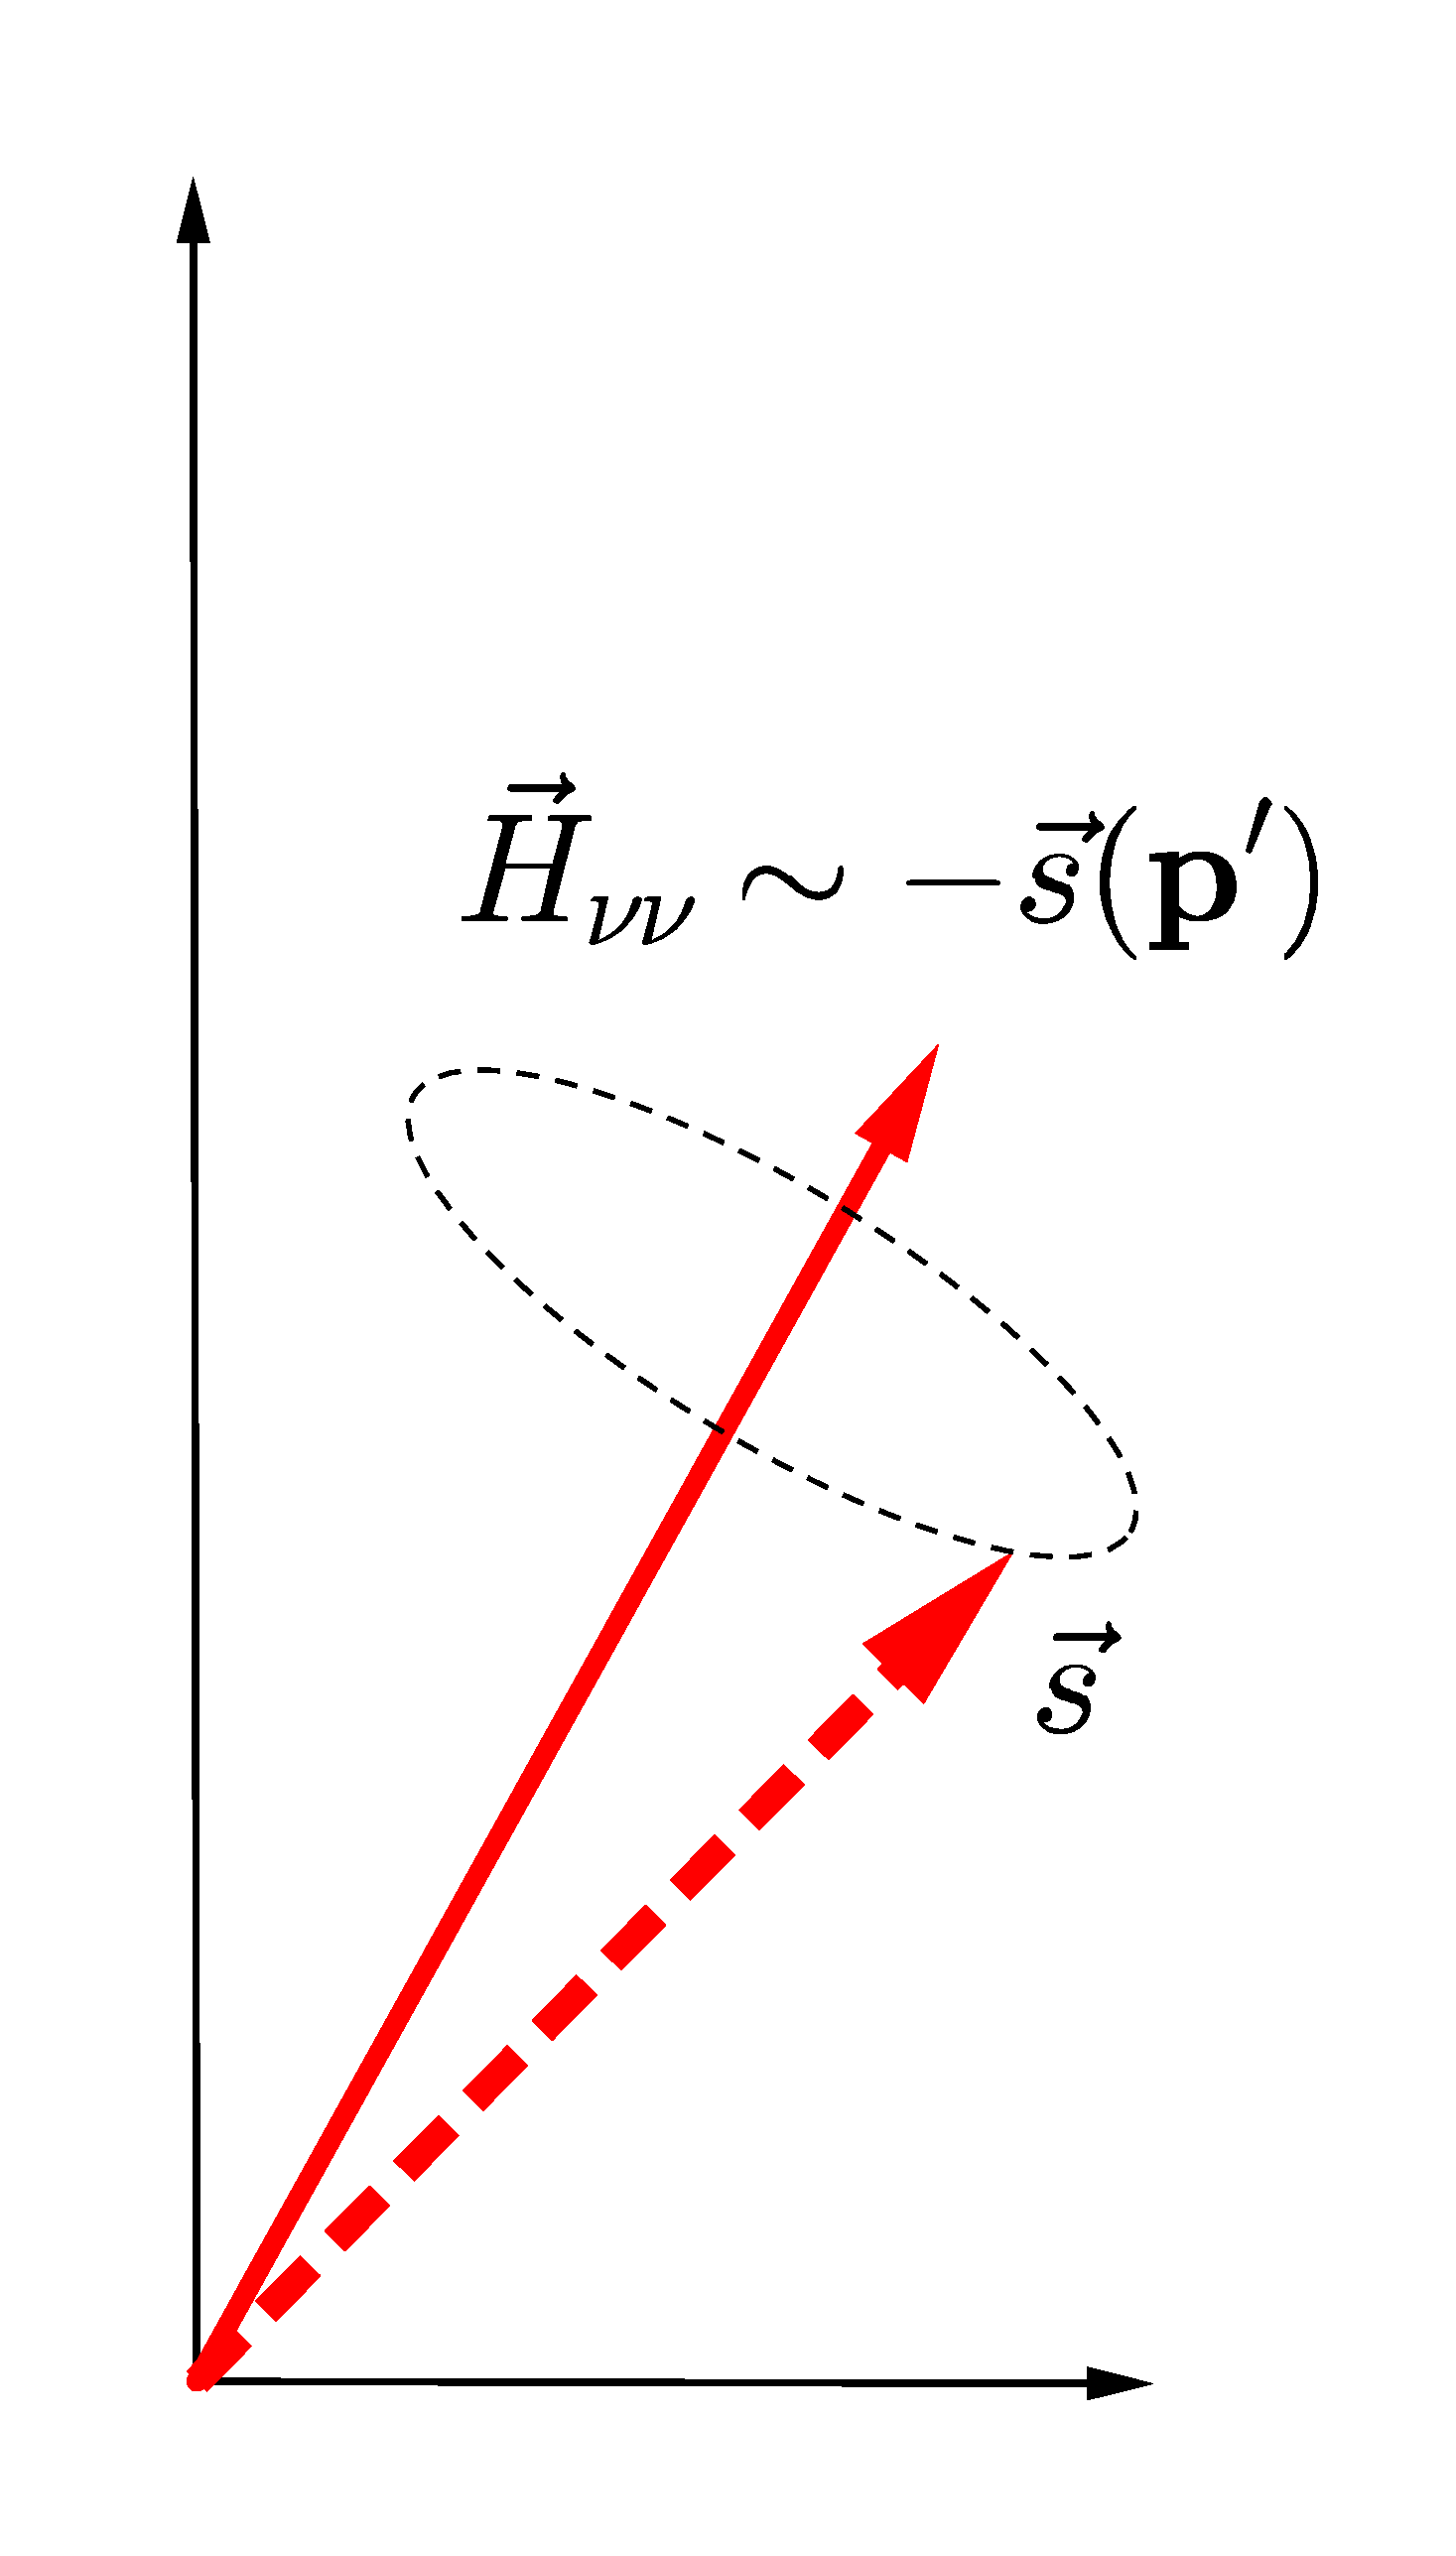
\includegraphics[width=0.4\textwidth]{chapters/assets/matter/self-interaction}
%     \caption{ Flavor isospin $\vec s$ precess around the Hamiltonian $\vec H_{\nu\nu}$ in flavor isospin space.}
%     \label{chap:collective-sec:collective-fig:self-interaction}
%  \end{figure}


% For single energy or flavor isospins aligned in the same direction, this vector is in the direction of the flavor isospin vector. If the flavor isospins are initially prepared in completely random and uniformly distributed directions, $\vec D\sim 0$.

% Synchronization occurs when the neutrino number density becomes large. $\vec D$ will wobble around very fast due to the precessions of flavor isospins, but almost stays in one direction. All the spins precess with the same frequency which is determined by $\mu$.

% With vacuum contribution $\vec H_{\mathrm v}$ and matter contribution $\vec H_{\mathrm m}$ to the Hamiltonian, we expect $\vec D$ to precess around $\vec H_{\mathrm v} + H_{\mathrm v}$, if the precession frequency of flavor isospins around $\vec D$ is much larger than the precession frequency of $\vec D$ around  $\vec H_{\mathrm v} + H_{\mathrm v}$.



\section{\label{chap:collective-sec:two-beams}Two-Beam Model and Flavor Instability}

During the synchronized flavor transformation, the whole neutrino medium behaves as if there were a single neutrino oscillates with the mean frequency $\langle \omega_\vv \rangle$ in vacuum. Under certain conditions, the neutrino self-interaction potential can cause the neutrino medium to evolve in a way completely different than the vacuum oscillations. I will illustrate this phenomenon using the two-beam neutrino model.

In the two-beam model, neutrinos and antineutrinos are emitted in two different directions from a plane (which we assume to be the $x$-$y$ plane) with angles $\theta_1$ and $\theta_2$ as shown in Fig.~\ref{chap:collective-sec:two-beams-fig:two-beam-line-model}. I will assume that the neutrino emission plane is homogeneous and that the neutrino and antineutrino have the same density $n$ in the emission plane. I will also assume that the matter density vanishes everywhere in space.



\begin{figure}[!htbp]
    \centering
    % 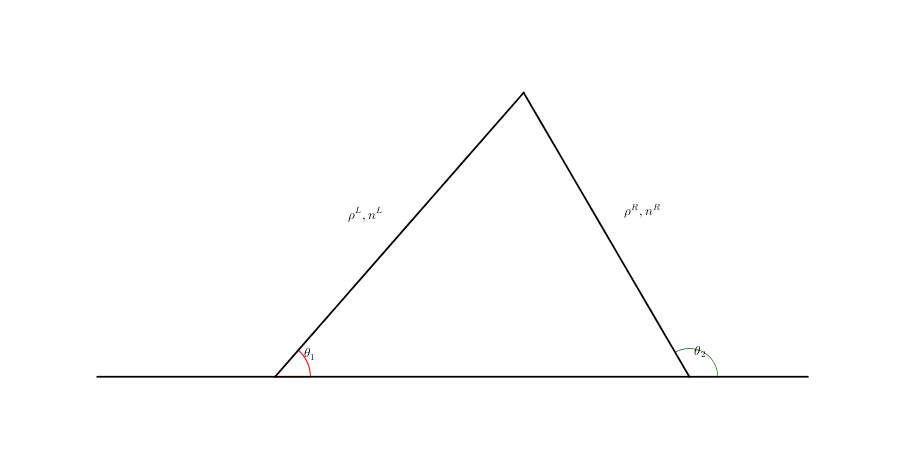
\includegraphics[width=\textwidth]{chapters/assets/dr/two-beam-line-model}
    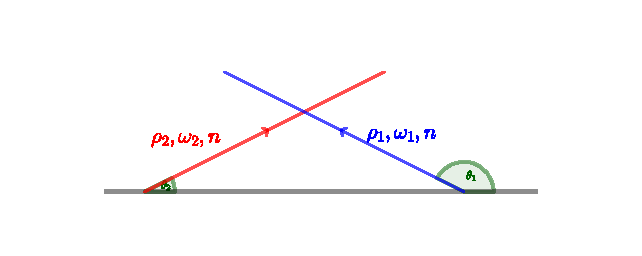
\includegraphics[width=\textwidth]{chapters/assets/collective/two-beams-model-sym}
    \caption{The geometry of two-beam model. The $i$th ($i=1,2$) neutrino beam has emission angle $\theta_i$, vacuum oscillation frequency $\omega_i$ and density matrix $\rho_i$. Both neutrino beams have the same number flux $n$.}
    \label{chap:collective-sec:two-beams-fig:two-beam-line-model}
\end{figure}


The Hamiltonian of the $i$th neutrino beam in the vacuum basis is 
\begin{align}
   \mathsf H_i &= -\frac{\omega_i}{2}  \sigma_3 + \mu ( \rho_1 -  \rho_2),
\end{align}
where $\omega_1 = \eta\omega_\vv$ for the neutrino beam and $\omega_2=-\eta\omega_\vv$ for the antineutrino beam,
\begin{align}
   \mu = \sqrt{2} G_{\mathrm F}  (1 - \cos(\theta_1 - \theta_2))  n
\end{align}
is the neutrino self-interaction potential.

I will assume that the neutrinos and antineutrino are emitted in the pure electron flavor at $z=0$. I will also assume the vacuum mixing angle $\theta_\vv \ll 1$. Therefore, the flavor density matrix of the $i$th neutrino beam in the vacuum basis at $z=0$,
\begin{equation}
    \rho_i (z=0)  \approx  \begin{pmatrix}
        1 & \epsilon_i (0) \\
        \epsilon_i^* (0) & 0
    \end{pmatrix},
    \label{chap:collective-sec:two-beams-eqn:density-matrix-perturbed}
\end{equation}
where
\begin{equation}
    \epsilon_i(0) = \sin (2\theta_\vv) \ll 1.
\end{equation}

I solve the two-beam model numerically with $\epsilon_i = 10^{-3}$ and $\eta=-1$. The solution is shown in Fig.~\ref{chap:collective-sec:two-beams-fig:two-beam-line-model-numerical-solution}. When $\omega_\vv z \ll 1$, the flavor isospin of the neutrino stays in the electron flavor state, i.e., in the direction of third axis $\vec e_3$ in the flavor isospin space (see the left panel of Fig.~\ref{chap:collective-sec:two-beams-fig:two-beam-line-model-numerical-solution}). Accordingly, the electron flavor survival probability $P_{\nu_\ee}\approx 1$ at small $z$ but falls down rapidly at a certain value of $z$ (see the right panel of Fig.~\ref{chap:collective-sec:two-beams-fig:two-beam-line-model-numerical-solution}). Then both the flavor isospin and $P_{\nu_\ee}$ come back to their original positions until they fall down again. The flavor isospin of the antineutrino follows a similar pattern but is in a different direction. This flavor transformation phenomenon is clearly different from the vacuum oscillation shown in Fig.~\ref{chap:basics-section:neutrinos-fig:vacuum-2-flavor-osc}.

\begin{figure}[!htbp]
    \centering
    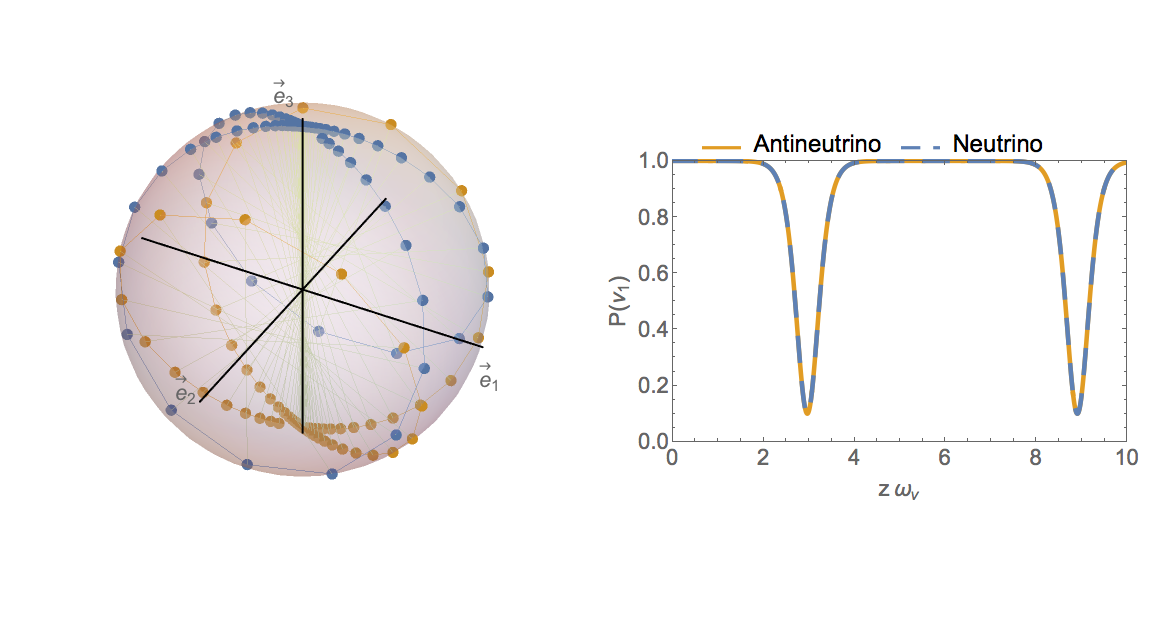
\includegraphics[width=\textwidth]{chapters/assets/collective/bipolar-animie100}
    \caption{The numerical solution to the two-beam model. The left panel shows the position of the flavor isospin of the neutrino beam (in blue) and the antineutrino beam (in orange). The right panel shows the probabilities as functions of distance $z$ (in unit of $\omega_\vv^{-1}$) for the neutrinos and antineutrinos to remain in the $\ket{\nu_1}$ and $\ket{\bar\nu_1}$ states, which are the same as the survival probabilities of the electron flavor when mixing angle $\theta_\vv \ll 1$. In this calculation, the emission angles are $\theta_1=5\pi/6$ and $\theta_2=\pi/6$, the neutrino self-interaction potential is $\mu=5 \omega_\vv$, and the neutrino mass hierarchy is inverted. }
    \label{chap:collective-sec:two-beams-fig:two-beam-line-model-numerical-solution}
\end{figure}

To gain a deeper understanding of the collective oscillation phenomenon, I will focus on the linear regime where $\lvert \epsilon_i(z) \rvert \ll 1$. The equation of motion is linearized in this regime and becomes
\begin{equation}
    \ri \partial_z \begin{pmatrix}
        \epsilon_1 \\
        \epsilon_2
    \end{pmatrix} =  \begin{pmatrix}
        \mu + \eta\omega_\vv & - \mu \\
        \mu & - \eta\omega_\vv - \mu
    \end{pmatrix} \begin{pmatrix}
        \epsilon_1 \\
        \epsilon_2
    \end{pmatrix}.
\end{equation}
This equation has two normal modes with corresponds to the collective modes of neutrino oscillations:
\begin{equation}
    \begin{pmatrix}
        \epsilon_1 (z) \\
        \epsilon_2 (z)
    \end{pmatrix} = \begin{pmatrix}
        Q_{1\pm} \\
        Q_{2\pm}
    \end{pmatrix} e^{i K_{z\pm} z},
    \label{chap:collective-sec:two-beams-eqn:equation-of-motion-collective-mode-assumption}
\end{equation}
where $(Q_{1\pm}, Q_{2\pm})^{\mathrm T}$ are the eigenvectors of the two normal modes, and 
\begin{equation}
    K_{z\pm} = \pm \sqrt{ \omega_\vv (\omega_\vv + 2 \eta \mu) }
\end{equation}
are the wavenumbers of the corresponding modes. For the normal mass hierarchy, $\eta = 1$, and $K_{z\pm}$ are always real. In this case, the electron flavor probability $P_{\nu_\ee}$ is always approximately 1. However, for the inverted neutrino mass hierarchy, $\eta=-1$, and $K_{z\pm}$ are imaginary when $\mu > \omega_\vv/2$. The normal mode with wavenumber $K_{z-}$ is a runaway solution which explains the rapid decrease of $P_{\nu_\ee}$ in Fig.~\ref{chap:collective-sec:two-beams-fig:two-beam-line-model-numerical-solution}.




% The linearized equation of motion becomes
% \small\begin{align}
%    &\ri \partial_z \begin{pmatrix}
%    \epsilon_1 \\
%    \epsilon_2
%    \end{pmatrix} =  - i \begin{pmatrix}\cot\theta_1\partial_x & 0 \\
%    0 & \cot\theta_2 \partial_x
%    \end{pmatrix} \begin{pmatrix}
%    \epsilon_1 \\
%    \epsilon_2
%    \end{pmatrix} + \nonumber\\
%    &
%    \frac{1}{2}\begin{pmatrix}
%    (\lambda+ \mu_2 - \eta \omega_1 - \mu_2 \cos(\theta_1-\theta_2) )/\sin \theta_1 & -\mu_2 (1-\cos(\theta_1-\theta_2)) /\sin \theta_1\\
%    -\mu_1 (1- \cos(\theta_1-\theta_2))/\sin\theta_2 & (\lambda + \mu_1 - \eta \omega_2 - \mu_1 \cos(\theta_1-\theta_2) )/\sin\theta_2
%    \end{pmatrix}\begin{pmatrix}
%    \epsilon_1 \\
%    \epsilon_2
%    \end{pmatrix},
%    \label{chap:collective-sec:two-beams-eqn:line-model-two-beams-all-neutrino-linearized-eom}
% \end{align}\normalsize
% where
% \begin{align*}
%    \mu_1 =& \sqrt{2}G_F n_{t,1}\\
%    \mu_2 =& \sqrt{2}G_F n_{t,2}.
% \end{align*}



% \subsection{Left-right Symmetric Emission}


% We first consider a simple case, where $\theta_1=\pi-\theta_2\equiv\theta$, $\lambda=0$, $\eta=1$, and homogeneous in $x$ direction. For simplicity we define
% \begin{align*}
%    \mu =& \sqrt{2}G_F (n_1 + n_2)\\
%    \mu_i =& \mu \frac{n_i}{n_1+n_2}\equiv \mu f_i \\
%    \xi = & 1-\cos(\theta_1-\theta_2) \\
%    \omega'_i = & \lambda - \eta\omega_i.
% \end{align*}

% % I am aware that this is not a self-consistent example since $\theta_1=\theta_2$ indicates that $\xi=0$. As we will see, no instability is present in this case. However, we keep the term $\xi$ because we need to analyze the effect of symmetry breaking. This example builds up a formalism.

% The equation for perturbations becomes
% \begin{equation}
%    i\partial_z\begin{pmatrix}
%    \epsilon_1 \\
%    \epsilon_2
%    \end{pmatrix} = \frac{1}{2\sin\theta} \begin{pmatrix}
%    \omega'_1 + \mu f_2\xi & -\mu f_2 \xi \\
%    -\mu f_1 \xi & \omega'_2 + \mu f_1 \xi
%    \end{pmatrix}\begin{pmatrix}
%    \epsilon_1 \\
%    \epsilon_2
%    \end{pmatrix}.
%    \label{eqn-linearized-eom-symmetric-eg}
% \end{equation}
% Since $\mu$ is the most important energy scale in this problem, we scale all energies with it.
% \begin{equation}
%    i\partial_{\hat z}\begin{pmatrix}
%    \epsilon_1 \\
%    \epsilon_2
%    \end{pmatrix} = \frac{1}{2\sin\theta} \begin{pmatrix}
%    \hat\omega'_1 +  f_2\xi & - f_2 \xi \\
%    - f_1 \xi & \hat\omega'_2 +  f_1 \xi
%    \end{pmatrix}\begin{pmatrix}
%    \epsilon_1 \\
%    \epsilon_2
%    \end{pmatrix},
% \end{equation}
% where
% \begin{align*}
%    \partial_{\hat z} =& \frac{d}{\mu dz} \\
%    \hat \omega'_i =& \frac{\omega'_i}{\mu}.
% \end{align*}


% The characteristic equation for this equation is
% \begin{equation}
%    \left( ( \Omega - \hat\omega'_1 - f_2\xi )(\Omega - \hat\omega'_2-f_1\xi) - f_1 f_2 \xi^2 \right) =0,
%    \label{chap:collective-sec:two-beams-eqn:two-beam-line-characteristic-eqn-simple}
% \end{equation}
% which is simplified to
% \begin{equation*}
%    (\Omega-\Omega_1)(\Omega-\Omega_2) -f_1f_2\xi^2 = 0,
% \end{equation*}
% where
% \begin{align*}
%    \Omega_1 = & \hat\omega'_1 + f_2 \xi\\
%    \Omega_2 = & \hat\omega'_2 + f_1 \xi.
% \end{align*}
% Complete the square
% \begin{equation*}
%    (\Omega - (\Omega_1 + \Omega_2)/2)^2 = \frac{1}{4}(\Omega_1-\Omega_2) + f_1f_2\xi^2.
% \end{equation*}
% The solution becomes
% \begin{equation}
%    \Omega = \frac{1}{2}(\Omega_1+\Omega_2)\pm\sqrt{ (\Omega_1-\Omega_2)^2/4 + f_1f_2\xi^2 }.
% \end{equation}
% The condition to have positive imaginary part is
% \begin{equation*}
%    (\Omega_1-\Omega_2)^2 + 4f_1f_2\xi^2 < 0,
% \end{equation*}
% or
% \begin{equation*}
%    -2\sqrt{-f_1f_2\xi^2}<\Omega_1-\Omega_2<2\sqrt{-f_1f_2\xi^2},
% \end{equation*}
% and $f_1f_2\xi^2<0$. Recall the meaning of $f_i$,
% \begin{equation*}
%    f_i = \frac{n_i}{n_1+n_2},
% \end{equation*}
% instability requires that we have a spectrum crossing, i.e., $n_1$ and $n_2$ have different signs. Plug in the definitions of $\Omega_i$,
% \begin{equation*}
%    -2\sqrt{-f_1f_2\xi^2}< \eta(- \omega_1 + \omega_2)/\mu + (f_2 - f_1)\xi < 2\sqrt{-f_1f_2\xi^2}.
% \end{equation*}
% From this we can infer
% \begin{itemize}
%     \item $f_1f_2$ has to be negative, which means we can NOT have instabilities with only neutrinos or antineutrinos with all the symmetries we assumed. This is crossing.

% \item $-\omega_1+\omega_2=0$ will remove the instability. So we have to have both neutrinos and antineutrinos.
% \item $f_2-f_1$, $\eta(\omega_2-\omega_1)$, and $\mu$ set limit on each other.
% \item $\theta_1=\theta_2\equiv \theta$ removes the instability since it leads to $\xi=0$. The emission has to be asymmetric in this simple two beams model. This is trivial since equal emission angle means the beams are not colliding.
% \end{itemize}


% % .. admonition:: But why?
% %   :class: warning

% %   We have these conclusions. But why?

% %   What are the roles of

% %   1. :math:`f_i`,
% %   2. neutrino beam and antineutrino beam,
% %   3. hierarchy,
% %   4. neutrino number density variations,
% %   5. variations of angular distributions of neutrinos,
% %   6. variations of energy spectrum of neutrinos.


% Another way of understanding this equation is to think of it as the growth of the length of the vector $\vec v = (\epsilon_1,\epsilon_2)^T$. For an arbitrary matrix differential equation of the form
% \begin{equation*}
%   \partial_z \mathbf v = \mathbf A \mathbf v,
% \end{equation*}
% we can always decompose the matrix $\mathbf A$ into symmetric part and skew-symmetric part
% \begin{equation*}
%   \mathbf A = \frac{1}{2}(\mathbf A + \mathbf A^T) + \frac{1}{2}(\mathbf A - \mathbf A^T) \equiv \mathbf A^+ + \mathbf A^-.
% \end{equation*}
% We can identify the effect of $f_1-f_2$ but this is not particularly useful since we can not say anything about the eigenvalues of matrix $\mathbf A$ from the eigenvalues of matrix $\mathbf A^+$ and $\mathbf A^-$.



% \subsection{Breaking Symmetries}



% For a line model, the symmetries we have are
% \begin{itemize}
%     \item Time translation symmetry;
% \item Translation symmetry along the line;
% \item Energy spectrum of the beams; One of particular interest is to have different neutrino spheres for different energies which can be investigated using two beam model.
% \item Number density of left and right beams;
% \item Angle of left and right beams;
% \item With and without matter.
% \item Similar to the discussion of varying matter potential, symmetries can be broken globally, i.e., distribution as a function of spacetime coordinates.
% \end{itemize}

% I will discuss some of the symmetries mentioned above.



% \subsubsection{Emission Angle Parity Symmetry}

% The emission angles change the value of $\xi=1-\cos(\theta_1-\theta_2)$ as well as rescale the quantities by angle dependent factor $1/\sin\theta_i$.

% To see the importance of angles, we can redefine some quantities
% \begin{align*}
%    \omega''_i=& \frac{\omega'_i}{\sin\theta_i}\\
%    f''_1=&\frac{f_1}{\sin\theta_2} \\
%    f''_2=&\frac{f_2}{\sin\theta_1}.
% \end{align*}
% The we will reach the same characteristic equation as Eqn. \ref{chap:collective-sec:two-beams-eqn:two-beam-line-characteristic-eqn-simple}. So the angles serves as shift of energy gap and angular distribution.

% The region of instability changes in a convoluted way. Given angles we can always write down the expression and find out.
% \begin{itemize}
%     \item  The criteria of existence of instability doesn't change.
% \item  The region of instability changes.
% \end{itemize}


% \subsubsection{Matter Effect}


% Including matter will define vacuum frequencies, $\omega'_i$, which is effectively just a shift of vacuum frequencies. In the symmetric emission case, $\omega'_1-\omega'_2$ is independent of matter effect. But breaking the emission symmetry generates the degeneracy,
% \begin{equation}
%    \hat\omega''_1-\hat\omega''_2=( \lambda/\sin\theta_1 - \lambda/\sin\theta_2 + \eta(- \omega_1/\sin\theta_1 + \omega_2/\sin\theta_2) )/\mu`.
% \end{equation}

% We notice that very large matter density shift the region to very small $\mu$.

% However, matter effect is not always this simple. Suppose we have different matter potential for different beams, when they collide they would have built a different phase due to matter effect.

% The inhomogeneous matter effect has been studied in \cite{Mangano2014}. It can excite high Fourier moments of flavor-isospin picture, which makes a lot of sense because it generates fine structure in the x direction. This might be integrated into LESA effect.



% \subsubsection{Translation Symmetry}


% Translation symmetry is better explained by introducing Fourier transform in x direction.

% For each mode, a term that is proportional to Fourier mode index $m$. It only appears in diagonal elements, thus is effectively a shift of vacuum frequencies, thus energies of neutrinos.

% For each Fourier mode
% \begin{equation*}
%    \begin{pmatrix}
%    \epsilon_1 \\
%    \epsilon_2
%    \end{pmatrix} =  \mathbf Q(\Omega,k) e^{-i(\Omega t- k x)},
% \end{equation*}
% where we set $\Omega=0$.

% First term in RHS of Eqn.~ \ref{chap:collective-sec:two-beams-eqn:line-model-two-beams-all-neutrino-linearized-eom} becomes
% \begin{equation*}
%    - i \begin{pmatrix}\cot\theta_1\partial_x & 0 \\
%    0 & \cot\theta_2 \partial_x
%    \end{pmatrix} \begin{pmatrix}
%    \epsilon_1 \\
%    \epsilon_2
%    \end{pmatrix} = k \begin{pmatrix}\cot\theta_1 & 0 \\
%    0 & \cot\theta_2
%    \end{pmatrix} \begin{pmatrix}
%    Q_1 \\
%    Q_2
%    \end{pmatrix}.
% \end{equation*}
% We now define $\hat\omega''_i$, so that
% \begin{equation*}
%    \hat\omega''_{k,i} = \hat \omega''_i + 2\hat k\cot\theta_i,
% \end{equation*}
% where $\hat k=k/\mu$.

% The $k$ term contributes to the difference between $\Omega_{k,i}\equiv \hat\omega''_{k,i}+ f''_i\xi$.

% We notice that instability criteria doesn't change. However, the regime of instability changes. We also know that the instability region is determined by
% \begin{equation}
%    \lvert \Delta\hat\omega''_{12} + 2\hat k (\cot \theta_1 - \cot\theta_2) + \Delta f''_{12}\xi \rvert < \sqrt{-f_1f_2\xi^2},
% \end{equation}
% where $\Delta \hat \omega''_{12} = \hat\omega''_1-\hat\omega''_2$. The instability region shift from
% \begin{equation}
%    -\sqrt{-f''_1f''_2\xi^2} -\Delta f''_{12}\xi < (\Delta\omega''_{12} + 2 k(\cot\theta_1-\cot\theta_2))/\mu < \sqrt{-f''_1f''_2\xi^2} -\Delta f''_{12}\xi
% \end{equation}
% If $\lvert \Delta\omega''_{12} + 2 k(\cot\theta_1-\cot\theta_2) \rvert$ becomes larger, the region of instability is shifted to larger $\mu$, i.e., larger number density.



% \subsubsection{Number Density of Emission}


% A crossing is required to have instability, i.e., $-f''_1f''_2>0$. Meanwhile the number density on the left and right have little effects on the existence of instability. It shifts the region of instability for $\mu$.


% \subsubsection{Energy of Emission}



% Different energy of two beams will make sure $-\omega_1 + \omega_2\neq 0$. It has no effects on the criteria but changes the $\mu$ region of instability.


% % \subsubsection{Time Translation Symmetry}



% % .. admonition:: Time Translational Symmetry
% %   :class: warning

% %   How about time translational symmetry? I need to write down the equation of motion that is related to time.

% %   Two limits are of particular interest.

% %   1. Adiabatic limit,
% %   2. Superfast time variants.



% For completeness, I can also write down the linearized equation of motion without translational symmetries, c.f.~Eqn.~\ref{chap:collective-sec:two-beams-eqn:line-model-two-beams-all-neutrino-linearized-eom}. I know that real symmetric matrix has only real eigenvalues, from which I infer that $\mu_1=\mu_2$ and $\theta_1=\theta_2$ removes the instability.
% For translation symmetric models, that is $\partial_x\to 0$, I have the eigenvalues
% \begin{equation*}
%    \Omega = \frac{1}{4}(A\pm B),
% \end{equation*}
% where
% \begin{align*}
%    A=& -\eta \omega_1/\sin\theta_1 - \mu_2 /\sin\theta_1 + \eta \omega_2 /\sin\theta_2 + \mu_1 \xi /\sin\theta_2 + \lambda(1/\sin\theta_1 + 1/\sin\theta_2)  \\
%    B=& \left(
%       -4[(\lambda-\eta\omega_1)(\lambda +\eta\omega_2) + (\lambda (\mu_1-\mu_2) -\eta (\mu_1\omega_1 + \mu_2\omega_2) )\xi ] \sin\theta_1 \sin\theta_2\right. \\
%       &\left.+ [(\lambda + \eta\omega_2 + \mu_1\xi) \sin\theta_1 + (\lambda - \eta \omega_1 - \mu_2\xi) \sin\theta_2 ]^2
%    \right)^{1/2}/(\sin\theta_1\sin\theta_2)\\
%    \xi=&1-\cos(\theta_1-\theta_2).
% \end{align*}


% For antineutrinos, I only need to change $\mu_i\to -\bar\mu_i$ and $\omega_i\to -\bar\omega_i$, where $\bar\mu=\sqrt{2}G_F \bar n_t$, so that the equation becomes
% \small\begin{align*}
%   &i \partial_z \begin{pmatrix}
%   \epsilon_1 \\
%   \epsilon_2
%   \end{pmatrix} =  - i \begin{pmatrix}\cot\theta_1\partial_x & 0 \\
%   0 & \cot\theta_2 \partial_x
%   \end{pmatrix} \begin{pmatrix}
%   \epsilon_1 \\
%   \epsilon_2
%   \end{pmatrix} \\
%   &+
%   \frac{1}{2}\begin{pmatrix}
%   (\lambda-\bar\mu_2 + \eta \bar\omega_1 + \bar\mu_2 \cos(\theta_1-\theta_2) )/\sin \theta_1 & \bar\mu_2 (1-\cos(\theta_1-\theta_2)) /\sin \theta_1 \\
%   \bar\mu_1 (1- \cos(\theta_1-\theta_2))/\sin\theta_2 & (\lambda -\bar\mu_1 + \eta \bar\omega_2 +\bar\mu_1 \cos(\theta_1-\theta_2) )/\sin\theta_2
%   \end{pmatrix}\begin{pmatrix}
%   \epsilon_1 \\
%   \epsilon_2
%   \end{pmatrix}
% \end{align*}\normalsize

% Assume that the left beam is neutrino beam and the right beam is antineutrno beam. The linearized equation of motion becomes
% \small
% \begin{align*}
%   &i\partial_z \begin{pmatrix}
%   \epsilon_1 \\
%   \epsilon_2
%   \end{pmatrix} =  -i\begin{pmatrix}
%   \cot\theta_1 \partial_x & 0 \\
%   0 & \cot\theta_2 \partial_x
%   \end{pmatrix}\begin{pmatrix}
%   \epsilon_1 \\
%   \epsilon_2
%   \end{pmatrix} \\
%   &+ \frac{1}{2}\begin{pmatrix}
%   (\lambda - \bar\mu - 2\eta \omega_1 + \bar\mu \cos(\theta_1-\theta_2) )/\sin\theta_1 & \bar\mu (1-\cos(\theta_1-\theta_2))/\sin\theta_1 \\
%   -\mu(1-\cos(\theta_1-\theta_2))/\sin\theta_2 & (\lambda + \mu + \eta \omega_2 - \mu \cos(\theta_1-\theta_2) )/\sin\theta_2
%   \end{pmatrix}\begin{pmatrix}
%   \epsilon_1 \\
%   \epsilon_2
%   \end{pmatrix}
% \end{align*}
% \normalsize







\section{\label{chap:collective-sec:fast-mode}Dispersion Relations}


The oscillation length scales of neutrino oscillations can be estimated by dimensional analysis. For example, the characteristic energy scale for vacuum oscillations is $\omega_{\mathrm v} = \delta m^2\big/2E $, which leads to neutrino oscillation frequency of the order
\begin{align*}
 \omega_{\mathrm v} = \frac{\Delta m^2}{2E}  \sim& \frac{2\pi}{ 1  \mathrm{km} }  \left(\frac{\Delta m^2_{32}}{2.5\times 10^{-3} \mathrm{eV}^2 } \right) \left( \frac{1MeV}{E} \right) \\
\sim & \frac{2\pi}{ 33  \mathrm{km} } \left( \frac{\Delta m_{12}^2}{7.5\times 10^{-5}\mathrm{eV}^2} \right) \left( \frac{1\mathrm{MeV}}{E} \right),
\end{align*}
where $E$ is the neutrino energy.
As for collective oscillations, suppose I have neutrino flux $10^{50}\mathrm{ergs\cdot s^{-1}}$. I can estimate the potential at radius $R$ to be
\begin{equation*}
\mu \sim  \frac{1}{0.01 \mathrm{km}} \left(\frac{100\mathrm{km}}{R}\right)^2 \left(\frac{1\mathrm{MeV}}{E}\right),
\end{equation*}
which means that the collective oscillations frequencies in supernova explosions can be much larger than the vacuum oscillations. The fast modes instability grows with a rate proportional to the neutrino potential $\mu=\sqrt{2}G_F n_\nu$, which is very large in dense neutrino media. In a paper by Chakraborty et al~\cite{Chakraborty2016}, they showed that neutrino oscillations in dense neutrino media can be much faster than than the vacuum oscillations.



% \subsection{\label{chap:collective-sec:fast-mode-subsec:introduction}Introduction}

% (Should talk about some very very basic backgrounds like the applications and why it is important.)





% \subsection{\label{chap:collective-sec:fast-mode-subsec:dr}Dispersion Relation of Neutrino Flavor Conversion}

In this section, I will review the dispersion relations by following the paper by I. Izaguirre, G. Raffelt, and I. Tamborra~\cite{Izaguirre2016a}.

I assume that all neutrinos and antineutrinos are emitted as electron flavor. The flavor evolution of neutrino ensemble depends on flavor density matrices of neutrinos $\rho$ and antineutrinos $\bar\rho$ with energy $E$, direction of velocity $\hat{\mathbf v}$,
\begin{equation}
\ii (\partial_t + \mathbf v\cdot \mathbf{\nabla}) \rho = \left[H, \rho_n \right],
\label{eqn-liouville-eqn}
\end{equation}
where $H$ is the Hamiltonian for neutrino oscillations. In the context, Hamiltonian depends on three different contributions from vacuum oscillations $H_{\mathrm v}$, interactions with matter $H_{\mathrm m}$, and interactions with neutrinos themselves $H_{\nu\nu}$. In this work, we ignore vacuum and matter terms since the concentration is on fast neutrino oscillations, which would occur even without neutrino mass differences \cite{Chakraborty2016,Dasgupta2017}. In order to calculate the neutrino self-interaction term $H_{\nu\nu}$, the distribution of neutrinos (antineutrinos) $f_{\nu_{\mathrm e}(\bar \nu_{\mathrm e})}(\hat{\mathbf v}, E)$ and $f_{\nu_{\mathrm x}(\bar \nu_{\mathrm x})}(\hat{\mathbf v}, E)$ is required, where $E$ is the energy of neutrinos (antineutrinos). We have
\begin{equation}
H_{\nu\nu} = \sqrt{2} G_{\mathrm F} n \iint \dd \Gamma' v^\mu v'_\mu \int \frac{E'^2 \mathrm d E'}{2\pi^2} \left( (f_{\nu_{\mathrm e}}' - f_{\nu_{\mathrm x}}' )\rho' -  (f_{\bar\nu_{\mathrm e}}' - f_{\bar\nu_{\mathrm x}}' ) \bar\rho' \right),
\end{equation}
where $v^\mu = ( 1, \sin\theta\cos\phi, \sin\theta\sin\phi, \cos\theta )^{\mathrm T}$ is the four velocity of (anti)neutrinos in our spherical coordinate system, and $\dd \Gamma' = \frac{\mathrm d \cos\theta' \mathrm d\phi'}{4\pi}$. Without vacuum contribution, the equation of motion for antineutrinos has the same form \cite{Duan2010}.

I follow the same assumption in reference \cite{Izaguirre2016a} that the the distribution of $\nu_x$ and $\bar\nu_x$ are the same, namely $ f_{\nu_{\mathrm x}}({\mathbf v},E)  - f_{\bar\nu_{\mathrm x}}({\mathbf v},E)=0$. In addition, I have the same definition of electron lepton number (ELN) of neutrinos travelling in direction ${\mathbf v}$ \cite{Izaguirre2016a},
\begin{equation}
G({\mathbf v}) =  \sqrt{2}G_{\mathrm F} n \int \frac{E'^2 \mathrm d E'}{2\pi^2} ( f_{\nu_{\mathrm e}}(\cos\theta',\phi',E')  - f_{\bar\nu_{\mathrm e}}(\cos\theta',\phi',E')  ).
\end{equation}
To perform linear stability analysis, I assume that the density matrix has the form
\begin{equation}
\rho = \bar \rho = \frac{1}{2} \begin{pmatrix}
1 & \epsilon \\
\epsilon^* & -1
\end{pmatrix},
\end{equation}
where $\lvert \epsilon \rvert \ll 1$. Plug this into the equation of motion, I obtain the linearized equation of motion
\begin{align}
    \ri ( \partial_t + \mathbf v \cdot \boldsymbol{\nabla} ) \begin{pmatrix}
        1 & \epsilon \\
        \epsilon^* & -1
        \end{pmatrix}  =  \left[ -\omega_\vv\sigma_3 + \int \dd \Gamma' G(\mathbf v') v^\mu v'_\mu  \begin{pmatrix}
            1 & \epsilon' \\
            \epsilon'^* & -1
            \end{pmatrix} , \frac{1}{2}\begin{pmatrix}
            1 & \epsilon \\
            \epsilon^* & -1
            \end{pmatrix}\right],
\end{align}
which leads to the equation for the perturbation
\begin{equation}
    \ri ( \partial_t + \mathbf v \cdot \boldsymbol{\nabla} ) \epsilon = v^\mu \Phi_\mu \epsilon - \int \dd \Gamma' v^\mu v'_\mu G(\mathbf v') \epsilon',
    \label{chap:collective-sec:fast-mode-eqn:eom-continuous-general-linearized}
\end{equation}
where I have assumed that all neutrinos and antineutrinos undergo the same behavior in linear regime, $\epsilon = \tilde\epsilon e^{-\ii (\Omega t - \mathbf K\cdot \mathbf x)}$. The four-potential in Eqn.~\ref{chap:collective-sec:fast-mode-eqn:eom-continuous-general-linearized}
\begin{equation}
    \Phi_\mu \to  \left( \int \dd \Gamma' G(\mathbf v'), \int \dd \Gamma' \mathbf v' G(\mathbf v') \right)^{\mathrm T}.
\end{equation}
With the equation of motion derived, I assume a collective mode 
\begin{equation}
\epsilon (t, \mathbf r) = \tilde \epsilon e^{- \ri (\Omega t - \mathbf K \cdot \mathbf r)},
\end{equation}
which is a generalization of Eqn.~\ref{chap:collective-sec:two-beams-eqn:equation-of-motion-collective-mode-assumption}. To get the equation of motion for the collective modes, I use the following substitution:
\begin{align}
    \epsilon & \to \tilde \epsilon, \\
    \partial_t & \to \ri \Omega, \\
    \boldsymbol{\nabla} & \to -\ri \mathbf K.
\end{align}
The equation of motion becomes
\begin{equation}
    v^\mu K_\mu \tilde \epsilon  = v^\mu \Phi_\mu \tilde \epsilon - \int \dd \Gamma' v^\mu v'_\mu G(\mathbf v') \tilde \epsilon',
\end{equation}
where $K_\mu \to (\Omega, \mathbf K)^{\mathrm T}$ is the four wave vector. I can combine $v^\mu K_\mu \tilde \epsilon$ and $v^\mu \Phi_\mu \tilde \epsilon$ by defining a new four wave vector
\begin{equation}
    k_\mu = K_\mu - \Phi_\mu.
\end{equation}
Following the convention of I. Izaguirre~\cite{Izaguirre2016a}, I define the polarization tensor.
\begin{equation}
\Pi^\mu_{\phantom{\mu}\nu} = 1 + \int \frac{\dd\cos\theta \dd \phi}{4\pi} G(\theta,\phi) \frac{v^\mu v_\nu}{\omega- k \hat{\mathbf k}\cdot \hat{\mathbf v} },
\end{equation}
which defines the dispersion relation $\Pi^\mu_{\phantom{\mu}\nu} a^\nu = 0$, with $a^\nu = \int \frac{d\cos\theta d\phi}{4\pi} G(\hat{\mathbf v}) v^\nu \tilde\epsilon$. I find the nontrivial solutions of the relation between $k_\mu$ by setting \cite{Izaguirre2016a},
\begin{equation}
\operatorname{det}\left( \Pi^\mu_{\phantom{\mu}\nu} \right) = 0.
\label{eqn-dr-determinant-equation}
\end{equation}


For simplicity, I consider axial symmetric neutrino emission so that Eqn.~\ref{eqn-dr-determinant-equation} becomes
\begin{align}
&\det \left( \omega \mathsf{I} + \frac{1}{2}
\begin{pmatrix}
   I_0 & 0 & 0 & -I_1 \\
   0 & -\frac{1}{2} (I_0 - I_2) & 0 & 0 \\
   0 & 0 & -\frac{1}{2} (I_0 - I_2) & 0 \\
   I_1 & 0 & 0 & -I_2
\end{pmatrix}\right) \nonumber\\
&=0,
\label{eqn-det-polarization-tensor-axial}
\end{align}
where $\mathsf I$ is the rank 4 identity matrix and
\begin{equation}
   I_m =\int_{-1}^{1} d u G(u) \frac{u^m}{1 -  \left(\lvert k\rvert /\omega\right) u }.
\end{equation}
where we define $u=\cos\theta$. Eq. \eqref{eqn-det-polarization-tensor-axial} is equivalent to the result in reference~\cite{Raffelt2013}. $\lvert k \rvert /\omega$ is defined as the refractive index $n$ of the flavor wave. For spectrum $G(u)$ without zero values, the forbidden region is given by $1 -  \left(\lvert k\rvert /\omega\right) u\leq 0$.

The dispersion relations can be categorized into two different types by symmetries. To incorporate azimuthal symmetry, I define solutions related to the first and second element of $a^\nu$ ($\nu=1,2$) to be multi-azimuthal angle (MAA) solutions since they are the only solutions that depend on azimuthal angle $\phi$. The other solutions which are related to $\nu=0,3$ are defined to be the multi-zenith angle (MZA) solutions. The MAA solution is related to symmetry breaking in azimuthal angle only, which is determined by
\begin{equation}
   \omega = \frac{1}{4}(I_0 - I_2).
   \label{eqn-maa}
\end{equation}
Similarly, the MZA solution is related to symmetry breaking in both azimuthal angle and zenith angle, which is
\begin{equation}
\omega = - \frac{1}{4} \left( I_0 - I_2 \pm \sqrt{ (I_0 + I_2 - 2 I_1) (I_0 + I_2 + 2 I_1) } \right).
\label{eqn-mza}
\end{equation}
I denote the solution associated with $+$ sign in Eq. \eqref{eqn-mza} as MZA+, while the solution assocated with $-$ sign as MZA-. The two solutions are connected to each other in dispersion relations. In general, it doesn't provide physical insights to distingush the two branches of solutions since they are simply two branches of the solution.

The solutions to Eq. \eqref{eqn-maa} and Eq. \eqref{eqn-mza} are dispersion relations $D(\omega,\mathbf k)$ for a chosen direction of $\hat{\mathbf k} = \hat{\mathbf z}$ with axial symmetric neutrino emission.



%%%%%%%%%%%%%%%%%
%% To BE Added
%%%%%%%%%%%%%%%%
% {\color{red}{\bf HAVE TO EXPLAIN THE IDEA OF GAP AND INSTABILITY HERE. Maybe Later?}}






\section{\label{chap:collective-sec:fast-mode-subsec:instabilities-and-gaps}Instabilities and Gaps}

In reference \cite{Izaguirre2016a}, the authors relate gaps in dispersion relation to instabilities of neutrino oscillations. In this section, I review the idea of correspondence betIen gaps and instabilities first. Then I show that this relation is not a solid theory that can be generalized to all cases.

I continue the discussion of axial symmetric neutrino emissions but with discretized zenith angles $\theta$ thus discretized $u$. Hence the ELN is independent of azimuth angle $\phi$. For neutrino emission with $2$ zenith angles, the ELN spectrum is
\begin{equation}
G(u)= \sum_{i=1}^2 g_i \delta(u - u_i)
\end{equation}

The MAA solution becomes an equation of hyperbola for $\omega$ and $k$, which has asymptotes $\omega = k u_i$ for $i=1,2$. Meanwhile, hyperbola equation has two solutions of $\omega$ ($k$) for any given real $k$ ($\omega$). The solutions are either real which indicates stable solutions or complex which indicates exponential growth or decrease in linear regime. On the other hand, non-existence of real solutions of $\omega$ ($k$) for given real $k$ ($\omega$) is equivalent to gap in dispersion relation. Thus the equivalence of gap and instabilities is guaranteed in neutrino emission with two-zenith-angle emission. The numerical calculations is normalized using the maximum value in spectrum which is a convention I follow for all discrete emission calculations. Unit for $\omega$ and $k$ can be determined once the exact spectrum is determined. Upper panels of Fig. \ref{fig-dr-db} is reproduction of left panels of Fig. 1 in reference \cite{Izaguirre2016a}. The dispersion relation is shown as black lines. The real part $\omega_{\mathrm R}$ is shown as red solid lines. $\omega_{\mathrm R} \pm \omega_{\mathrm I}$ are shown are red dashed lines, where $\omega_{\mathrm I}$ is the imaginary part of $\omega$.



\begin{figure}[!htb]
\minipage{0.49\textwidth}
  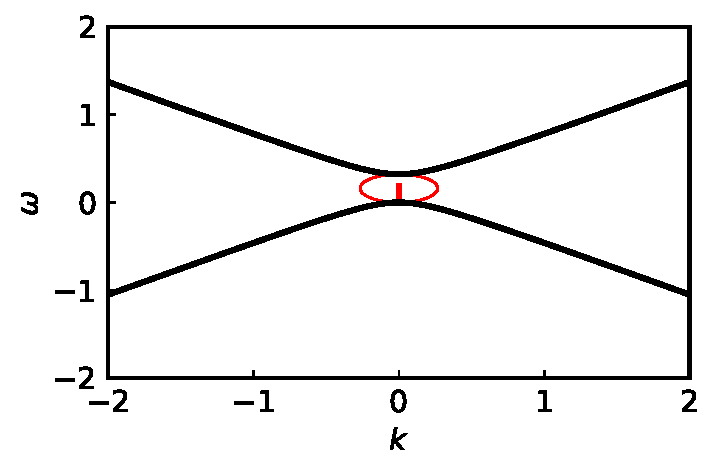
\includegraphics[width=\linewidth]{chapters/assets/dr/spectDBWC1DRDBMAAPltBlob.pdf}
\endminipage\hfill
\minipage{0.49\textwidth}
  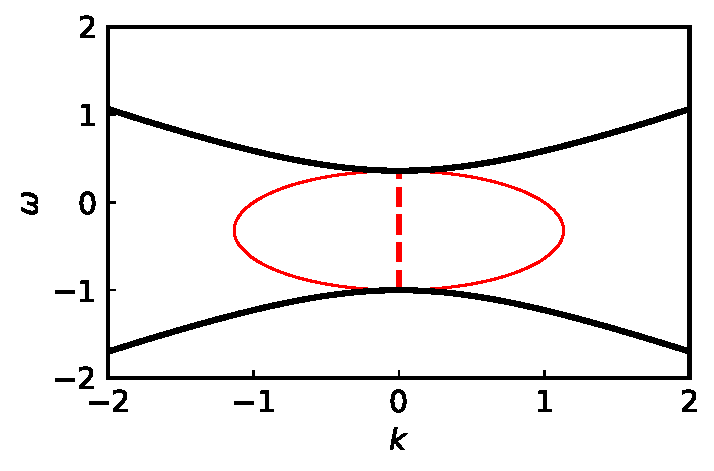
\includegraphics[width=\linewidth]{chapters/assets/dr/spectDBWC1DRDBMZAPltBlob.pdf}
\endminipage\hfill
\newline
\minipage{0.49\textwidth}
  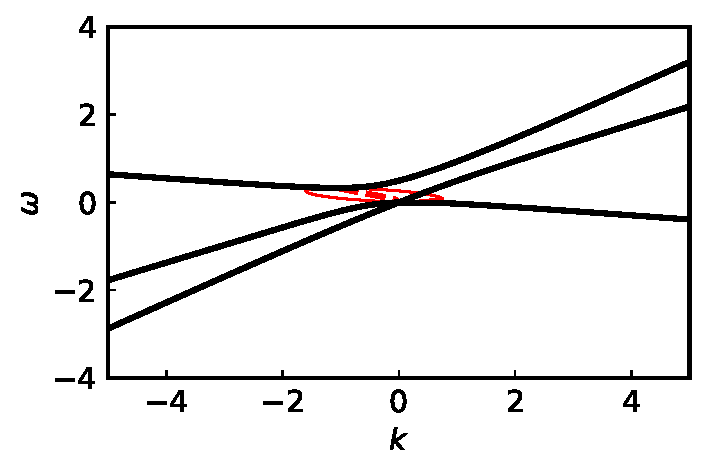
\includegraphics[width=\linewidth]{chapters/assets/dr/spectDB3WC4DRDBMAAPltBlob.pdf}
\endminipage\hfill
\minipage{0.49\textwidth}
  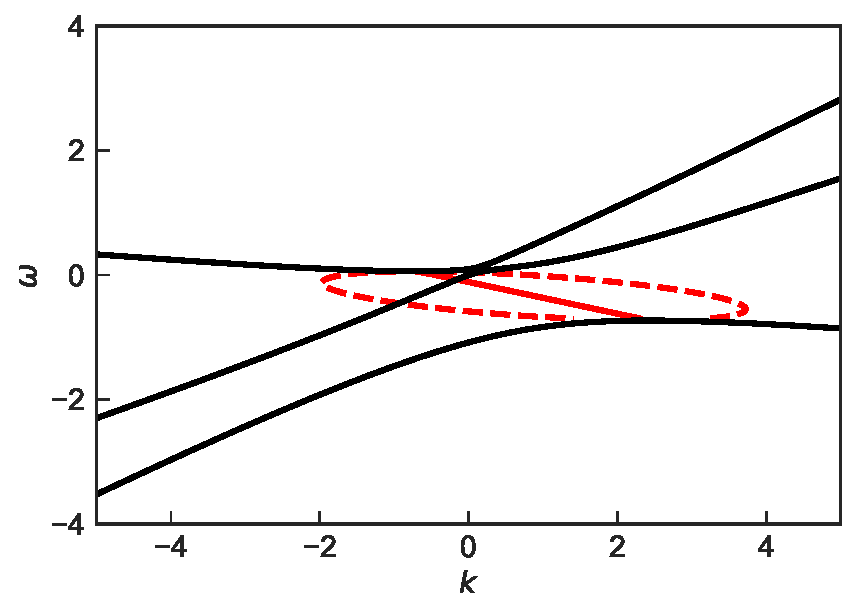
\includegraphics[width=\linewidth]{chapters/assets/dr/spectDB3WC4DRDBMZAPltBlob.pdf}
\endminipage\hfill
\caption{Dispersion relation and instabilities of two zenith angles spectrum (upper panels) and three zenith angles spectrum (loIr panels). The black lines are the dispersion relations and the colored dots are examples of complex $\omega$ for real $k$. The left panels are the dispersion relation and linear stability analysis of MAA solutions while the right panels are for MZA solutions.}
\label{fig-dr-db}
\end{figure}



In core collapse supernova and neutron star mergers, neutrino emission is not in discrete zenith angles. More realistic models involve continuous zenith angle ELN spectra. In the case that the smooth and continuous ELN spectrum has no crossing, gap indeed indicates instabilities, as shown in reference \cite{Izaguirre2016a}. In this section I prove that the instabilities in MAA, MZA+, or MZA- solution can only appear in either region $\omega\leq 0$ or region $\omega \geq 0$. As it suggests, the instability regions propagate only betIen the dispersion relation curves and the axis $\omega=0$. I reproduced the calculation in reference \cite{Izaguirre2016a} using the same Garching core-collapse supernova data set \cite{garching-ccsn-data}. The spectrum shown in the left panel of Fig. \ref{fig-garching} is polynomial fitting of the Garching 1D supernova simulation data. On the right of Fig. \ref{fig-garching}, the dispersion relation for MAA (MZA) solution is shown as red (green, blue) solid lines. Instabilities associated with MAA (MZA) solution is shown as light red (light green, light blue) blobs. The two branches of MZA solutions appear at the top half (MZA+) and lower half (MZA-). The result shows that instabilities occur either in region $\omega>0$ or region $\omega<0$ and with limits set the dispersion relation. Iwill prove that the instabilities appear between the dispersion relation and the axis $\omega=0$.






\begin{figure}
   \minipage{0.49\textwidth}
     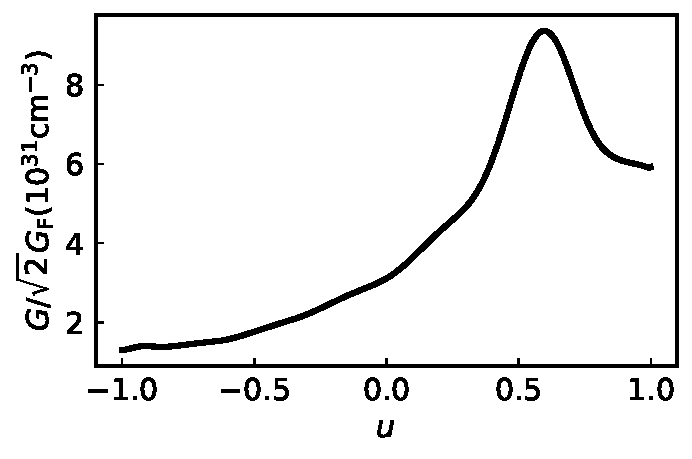
\includegraphics[width=\linewidth]{chapters/assets/dr/spectGarchingPlt.pdf}
   \endminipage\hfill
   \minipage{0.49\textwidth}
   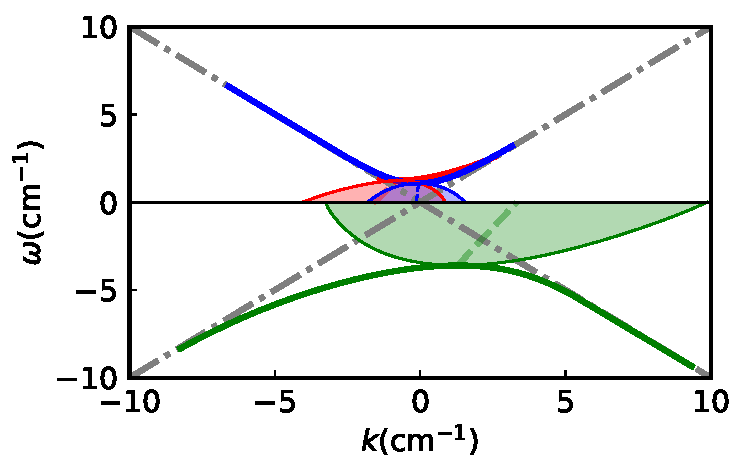
\includegraphics[width=\linewidth]{chapters/assets/dr/spectGarchingDRLSAPltBlob.pdf}
   \endminipage\hfill
   \caption{Dispersion relation and linear stability analysis (right panel) for a spectrum constructed from Garching 1D simulation data (left panel). Solid red line is dispersion relation for MAA solution while blue and green lines are for MZA solutions. Light red (green and green) blob is instability for MAA (MZA) solution.
    }
   \label{fig-garching}
\end{figure}




% \subsection{\label{sec-omega-to-zero}Instabilities at $\omega\to 0$}

Suppose I am looking for complex solutions for given real omega as in Fig. \ref{fig-garching}, MAA solution Eq. \eqref{eqn-maa} is rewritten as a function $k(\omega/k)$. More explicitly, I have to solve the integral function to find out $k$ for real $\omega$,
\begin{equation}
   k = \frac{1}{4} \int \mathrm du G(u) \frac{ 1 - u^2 }{ \omega/k - u }.
   \label{eqn-k-omega-relation}
\end{equation}
To investigate how instabilities developed around the horizental axies, I solve Eq. \eqref{eqn-k-omega-relation} in the limit $\omega\to 0$. For complex $k$, the integral can be decomposed into the principal value $\operatorname{Re}(k)$ and imaginary part $\operatorname{Im}(k)$ using Sokhotski–Plemelj theorem,
\begin{subequations}
\begin{align}
\operatorname{Re}(k) =& \frac{1}{4}\left(  \mathcal{P} \int \mathrm d u G(u) \frac{ 1 - u^2 }{ - u }  \right)\label{eqn-re-k-arbitrary-spectrum} \\
\operatorname{Im}(k) =&  \frac{\pi}{4}G(0) \operatorname{Sign}\left( \omega \right) \operatorname{Sign}\left(  \operatorname{Im}(k)  \right).
\label{eqn-im-k-arbitrary-spectrum}
\end{align}
\end{subequations}
Assuming no crossing is found in sepctrum $G(u)$ at $u=0$, Eq. \eqref{eqn-im-k-arbitrary-spectrum} shows that $\omega$ must have the same sign as $G(0)$ if I find nonzero imaginary part in $k$. I conclude that instabilities can only grow either in the upper plane $\omega>0$ or lower plane $\omega<0$. What's more, the value of $k$ at limit $\omega\to 0$ can be solved out of Eq. \eqref{eqn-re-k-arbitrary-spectrum} and Eq. \eqref{eqn-im-k-arbitrary-spectrum}. For instabilities the imaginary part of $k$ tells us the growth rate is,
\begin{equation}
   \lvert \operatorname{Im}(k) \rvert  =  \frac{\pi}{4}\lvert G(0)\rvert .
\end{equation}
Similar result is obtained for MZA solutions,
\begin{align}
&\left(4\operatorname{Re}(k) - \mathcal P \int \frac{G(u)}{u} \mathrm d u + U_1 \right)^2  - \left( \operatorname{Sign}(\omega \operatorname{Im}(k) )\pi G(0) +4 \operatorname{Im}(k) \right)^2 \\
% =&\left( \mathcal P \int \frac{G(u)}{u} \mathrm d u + U_1 \right)^2 -1 - 4 U_0^2  \\
% &\left( 4 \operatorname{Re}(k) - \mathcal P \int \frac{G(u)}{u} \mathrm d u + U_1 \right) \left( \pi \operatorname{Sign}(\omega \operatorname{Im}(k) ) G(0) + 4 \operatorname{Im}(k) \right) \\
=& - \left( \mathcal P \int \frac{G(u)}{u} \mathrm du + U_1 \right) \pi \operatorname{Sign}(\omega \operatorname{Im}(k) ) G(0),
\end{align}
where $U_m = \int G(u) u^m \mathrm du$ and all the integrals are over all the sepctrum. The equations are quadratic in both $\operatorname{Re}(k)$ and $\operatorname{Im}(k)$ so the real solutions can be calculated and verified with linear stability analysis. The imaginary part $\operatorname{Im}(k)$
\begin{equation}
   \operatorname{Im}(k) = - \frac{1}{4} \pi G(0) \operatorname{Sign}(\omega \operatorname{Im}(k) ) \left(  1 \pm \frac{ \mathscr P \int \frac{G(u)}{u} du + \int G(u) u du }{ 4 \operatorname{Re}(k) - \mathscr P \int \frac{G(u)}{u} du + \int G(u) u du }  \right)
\end{equation}
determines that the two different solutions are either in the region $\omega>0$ or in the region $\omega<0$ which corresponds to MZA+ and MZA- solutions. The instabilities in the two regions are not continuous at $\omega=0$.



\subsection{\label{chap:collective-sec:fast-mode-subsec:instability-to-gap}Instabilities Do Not Always Show Up as Gap}

Even though the concept of gap leads to instabilities works well for the models in \ref{chap:collective-sec:fast-mode-subsec:instabilities-and-gaps}, it can not be generalized to arbitrary number of emission angles nor to continuous spectra with crossings. As an example, I perform linear stability analysis of the three zenith angles emission configuration which is determined by a cubic function both in $\omega$ and $k$. Three solutions of $k(\omega)$ for given real $\omega(k)$  are expected. As long as real solutions disappear, complex solutions emerge, which leads to instabilities occur even without an actual gap. Rather the decrease in the number of real solutions for fixed $\omega$ or $k$ corresponds to the instabilities. As an example, I plotted dispersion relation and instabilities for three zenith angles in lower panels of Fig. \ref{fig-dr-db}. For a given value of $\omega$ such as $\omega= 0.5$, the three MAA solutions (Fig. \ref{fig-dr-db} lower left panel) of $k$ are $k=-4.6, 0.29, 1.2$. All three solutions are all real and indicate no spatial instabilities which is confirmed by calculation of instabilities shown as red blob. However, for another real $\omega = 0.2$, I find only one real solution $k=0.4$ from dispersion relation. The other solutions are complex and proven to be $k = -0.557106\pm 0.966535\mathrm i$ where the value with positive imaginary part leads to exponential growth. I conclude that instabilities doesn't require gap in dispersion relation except for two emission angles.


I will prove that instabilities for continuous emission angles do not necessarily correspond to gap in dispersion relation. In the earlier works of fast modes, Sawyer analyzed a box shaped angular distribution of neutrino emission \cite{Sawyer2016}. To address the generality of our conclusion, I repeat the calculation for box spectrum with crossing.

I construct a box spectrum with value $-0.1$ within $u\in [-1,-0.3)$ and value $1$ within $[-0.3,1]$ as shown in the top left panel of Fig. \ref{fig-box-c1}. As in the discrete emission case, I normalize all quantities using the maximium value of the spectrum. With the spectrum defined, I calculate the dispersion relation and find out complex values of $k$ for real $\omega$. The result shows that the dispersion relation of both MAA solution and MZA solution contains only one curve. No gap is formed but I observe instabilities between this curve and $\omega=0$ in MAA solution as well as two unstable regions of $k$ in MZA solution, which are plotted as red lines.


\begin{figure}
   % \minipage{0.49\textwidth}
   %   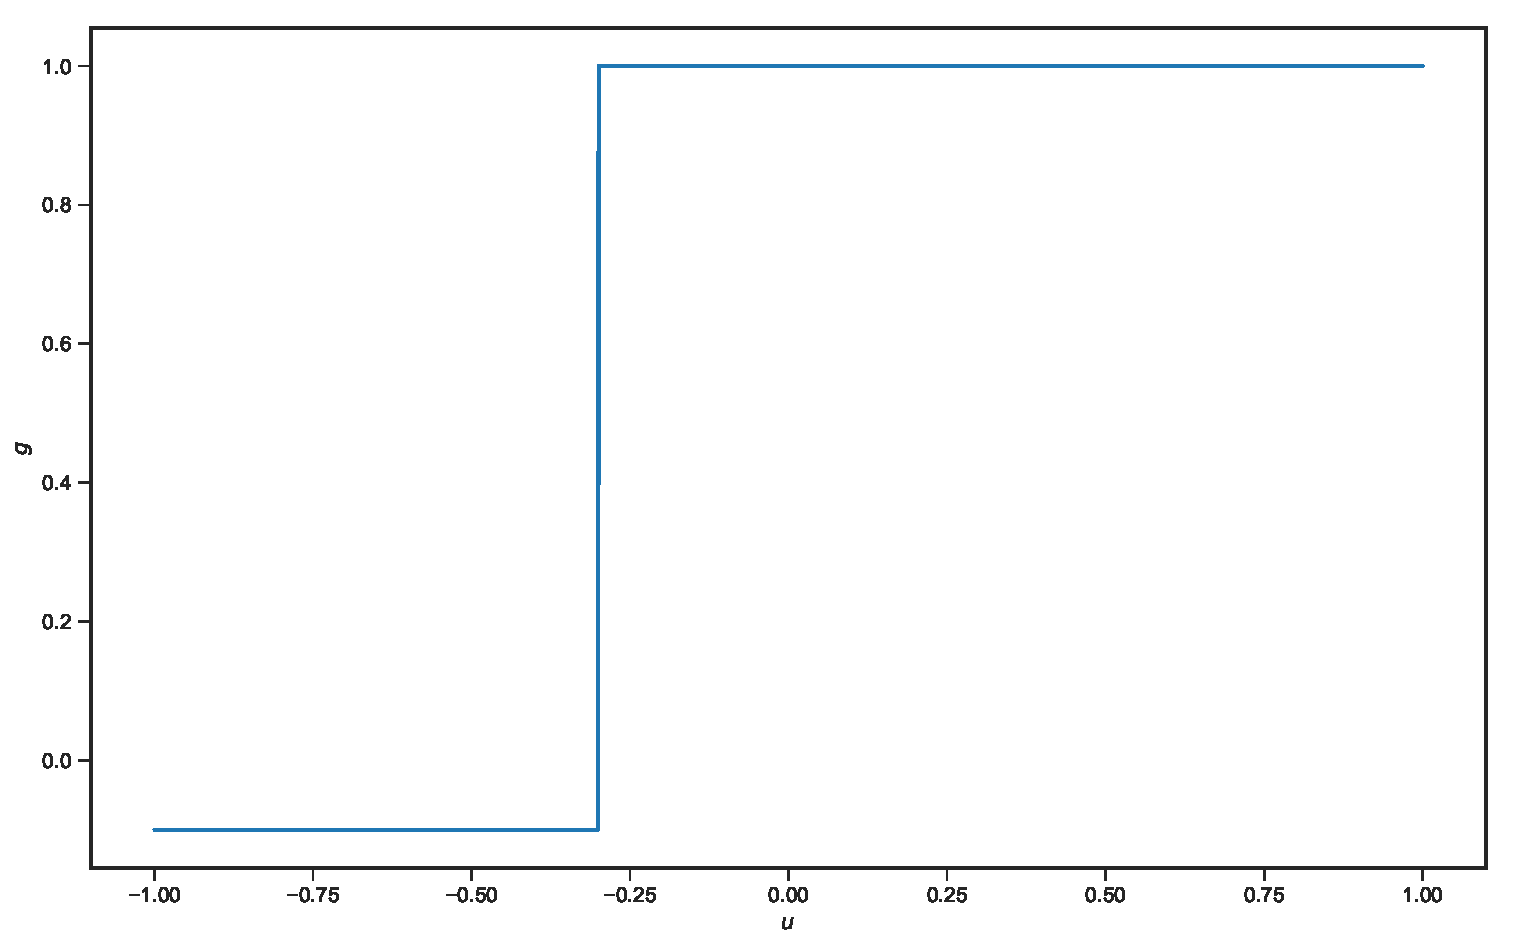
\includegraphics[width=\linewidth]{chapters/assets/dr/spectBoxC1Spectrum.pdf}
   % \endminipage\hfill
   \minipage{0.49\textwidth}
   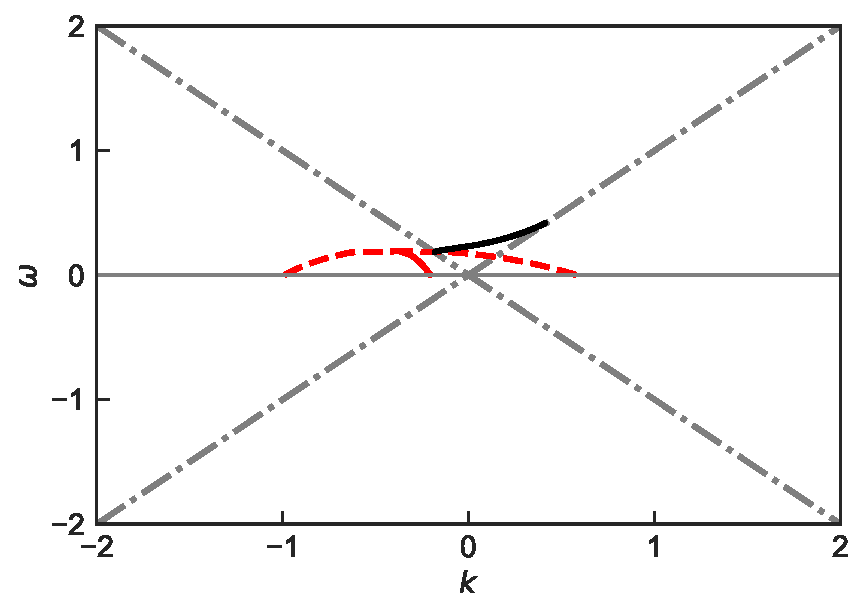
\includegraphics[width=\linewidth]{chapters/assets/dr/spectBoxC1MAADRPltBlob.pdf}
   \endminipage\hfill
   \minipage{0.49\textwidth}
   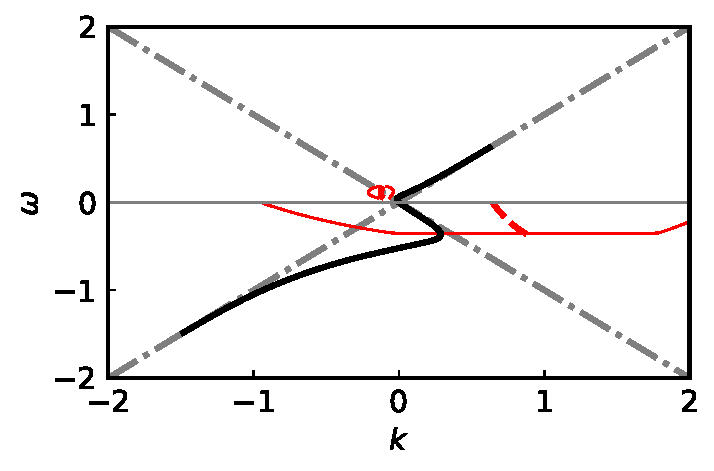
\includegraphics[width=\linewidth]{chapters/assets/dr/spectBoxC1MZADRPltBlob.pdf}
   \endminipage\hfill
   \caption{Dispersion relation and linear stability analysis for box spectrum. The box spectrum is defined to be $-0.1$ within range $u\in [-1,-0.3)$ and $1$ within range $u\in [-0.3,1]$. Left panel shows the dispersion relation and the complex $k$ for real $\omega$ for MAA solution. Right panel is the corresponding result for MZA solution. Dash-dotted gray lines are $\omega= \pm k$ which sets the boundaries of the forbidden region for dispersion relation.
    }
   \label{fig-box-c1}
\end{figure}



%%%%%%%%%%%%%%%%%%%%%%%%%%%%%%%%%%%%%%%%%%%%%%%%%%%%%%%%%%%%%%%%%%%%%%%%%
%%%%%%%%%%%%%%%%%%%%%% Neutrino Halo Problem %%%%%%%%%%%%%%%%%%%%%%%%%%%%
%%%%%%%%%%%%%%%%%%%%%%%%%%%%%%%%%%%%%%%%%%%%%%%%%%%%%%%%%%%%%%%%%%%%%%%%%





\section{\label{chap:halo}Neutrino Halo Problem}


One of the big questions about neutrino oscillations in supernovae is the so called halo problem. Cherry et al showed that neutrino flavor conversions are greatly affected by the back scattered neutrinos in supernovae~\cite{Cherry2012}. Neutrinos around supernovae are scattered and some of them are scattered to move almost backward. On the other hand, neutrino self-interactions is proportional to the inner product of momenta of neutrinos, which leads to the dependence on $1-\cos\theta$ where $\theta$ is the angles between momenta of two neutrinos. Most of the research has been concentrating on mostly forward scattering, with small values for $1-\cos\theta$. For back ward scattered neutrinos, the interaction potential can be much larger than the forward scattered neutrino contributions. Though the work by Sarikas et al showed that matter suppression is still significant within this region~\cite{Sarikas2012a}, it is not clear how exactly the neutrino halo alters neutrino oscillations. The halo problem itself is worth more calculations. In this chapter, I will present a relaxation method for this problem. The focus will be on the numerical method itself.


\subsection{\label{chap:halo-sec:line}Line Model}

I continue to use the simplified line model and build our intuitions out of it. The halo problem is simplified to have neutrinos emitted from a line $z=0$ homogeneously, which are reflected from a certain distance $z=L$. In principle, the reflection angles doesn’t have to be Snell’s law. The scattering can be in any angle with different amplitudes. Here I am using this very simple Snell’s law just to explore the effect of halo. It's crucial to keep an eye on the simplifications in this line model.
\begin{itemize}
    \item Neutrinos are emitted from a line, which is not the case in a real supernova.
    \item Neutrinos are emitted with translation symmetry on the line. Breaking the symmetry might bring in other qualitatively different results.
    \item Neutrinos are reflected from a certain surface $z=L$, which is different from reality where neutrinos are scattered everywhere.
    \item Neutrinos are reflected according to Snell's law.
    \item Neutrinos are homogeneously reflected at $z=L$.
\end{itemize}



\begin{figure}
    \centering
    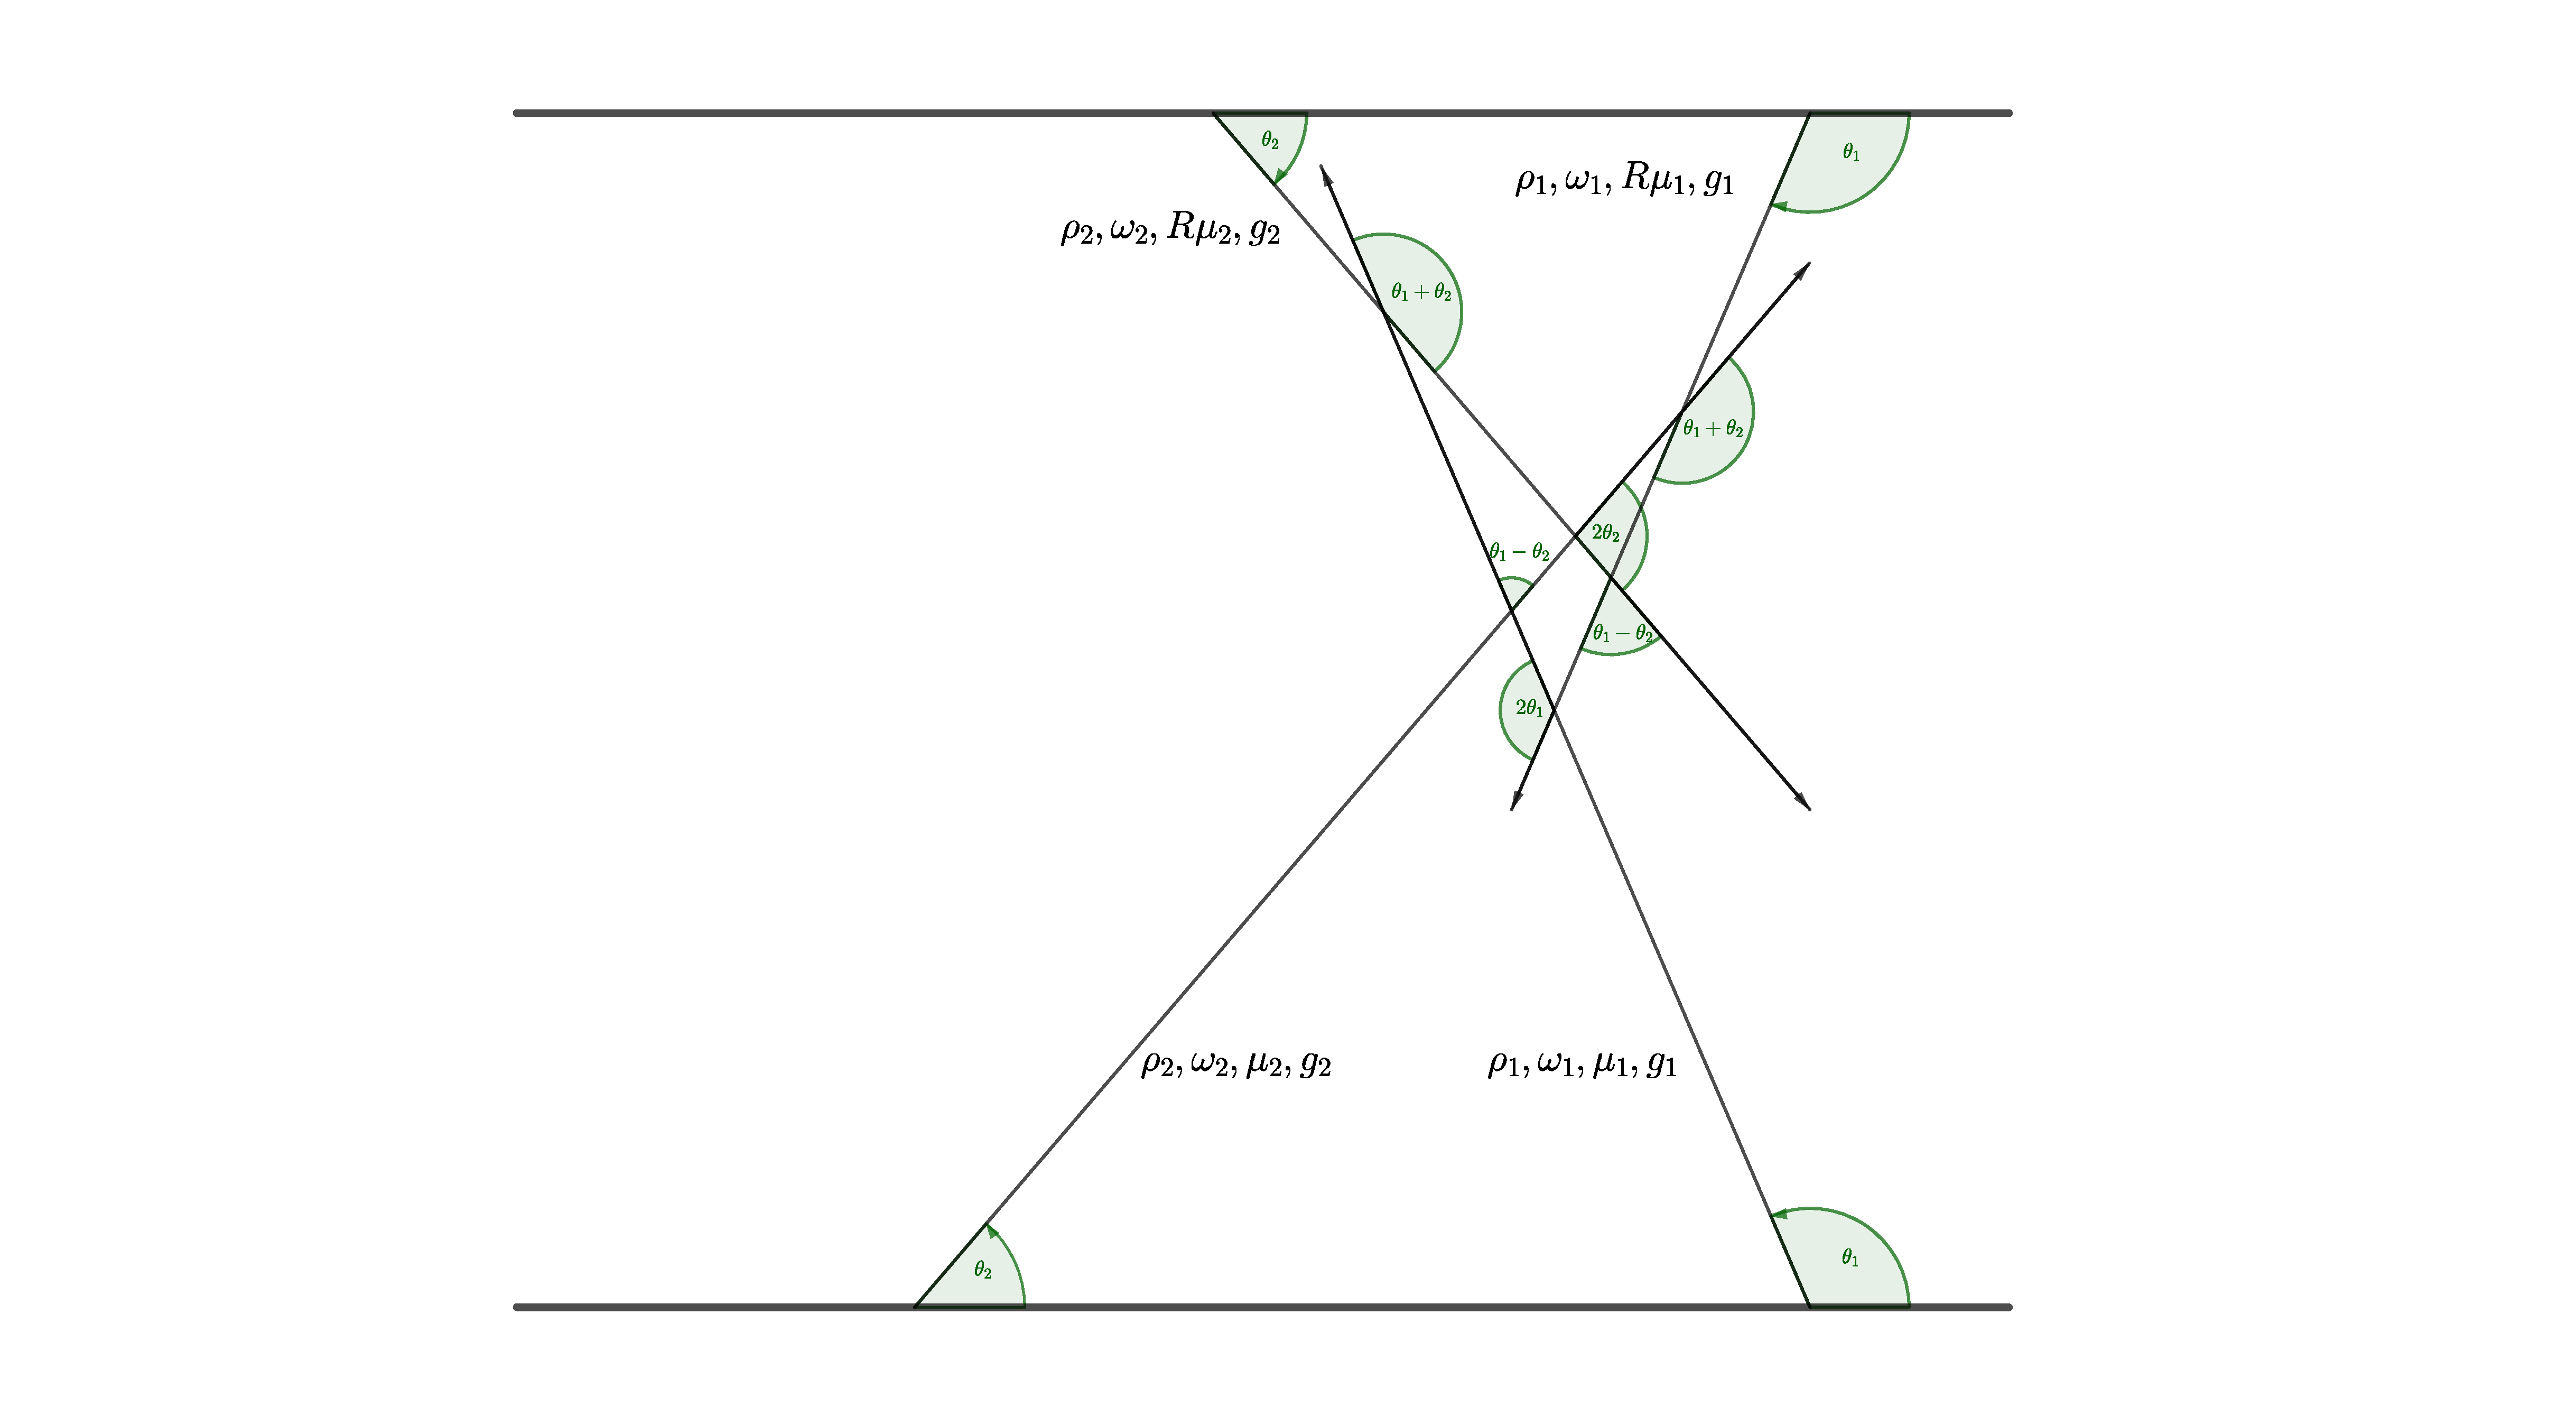
\includegraphics[width=\textwidth]{chapters/assets/halo/line-model.pdf}
    \caption{Line model used for halo problem. Neutrinos are emitted from the bottom line and reflected at the top line. Two neutrino beams are demonstrated in the figure. The beams are reflected from a surface at $z=L$.}
    \label{chap:halo-sec:line-fig:line-model}
\end{figure}


The algorithm that I used is relaxation method. The algorithm is meant to find the equilibrium state of neutrino oscillations with the presence of halo.
\begin{enumerate}
\item Calculate forward beam using 0 backward beam;
\item Calculate backward beam using forward beam calculated in 1;
\item Calculate forward beam using backward beam calculated in 2;
\item Repeat until the beams reach equilibrium.
\end{enumerate}


\subsection{\label{chap:halo-sec:line-sym}Neutrino Beams Only}

As a first step, I calculated neutrino oscillations with only neutrino beams. Before I rush to the numerical results, I linearized the equation of motion and worked out the linear stability analysis.

In linear regime, I define the density matrices for forward and backward beams to be
\begin{align*}
   \rho_F &= \frac{1}{2} \begin{pmatrix}
   1 & \epsilon_F \\
   \epsilon_B^* & -1
   \end{pmatrix} \\
   \rho_B &= \frac{1}{2} \begin{pmatrix}
   1 & \epsilon_B \\
   \epsilon_B^* & -1
   \end{pmatrix}.
\end{align*}
The Hamiltonian for forward and back ward beams are
\begin{align*}
   H_F &= H_v + R \mu \rho_B \\
   H_B &= H_v + \mu \rho_F.
\end{align*}
I will investigate the instability for zero mixing angle for new instabilities. The linearized equation of motion can be simplified to
\begin{align*}
   i\partial_z \begin{pmatrix}
   \epsilon_F \\
   \epsilon_B
   \end{pmatrix} = \begin{pmatrix}
   -\omega_v + R \xi \mu & - R \xi \mu \\
   \xi \mu & \omega_v - \xi \mu
   \end{pmatrix} \begin{pmatrix}
   \epsilon_F \\
   \epsilon_B
   \end{pmatrix}.
\end{align*}
This equation can be easily solved. The eigenvalues are
\begin{align*}
   \Omega_+ &= \frac{1}{2} ( (R-1)\xi\mu + \sqrt{\Delta} ) \\
   \Omega_- &= \frac{1}{2} ( (R-1)\xi\mu - \sqrt{\Delta} ),
\end{align*}
where
\begin{equation}
   \Delta = (1-R)^2 \mu^2 \xi^2 - 4\mu\xi \omega_v (1+R) + 4\omega_v^2.
\end{equation}
The corresponding eigenvectors are
\begin{align*}
   V_+ &=\begin{pmatrix}
   \frac{ -2\omega_v + \xi \mu (1+R) + \sqrt{\Delta} }{2\xi\mu} \\
   1
   \end{pmatrix} \\
   V_- &=\begin{pmatrix}
   \frac{ -2\omega_v + \xi \mu (1+R) - \sqrt{\Delta} }{2\xi\mu} \\
   1
   \end{pmatrix}.
\end{align*}
The general solution to the equation is
\begin{equation*}
   \begin{pmatrix}
   \epsilon_F(z) \\
   \epsilon_B(z)
   \end{pmatrix} = C_+ V_+ e^{-i \Omega_+ z} +  C_- V_- e^{-i \Omega_- z}.
\end{equation*}

The special property about this reflection problem is that the density matrices for the forward and backward beams should be the same at the reflection point, say $z=L$. With such a simple relation, we can find the relations between $C_\pm$ by setting $\epsilon_F(L)=\epsilon_B(L)$,
\begin{equation}
   \frac{C_+}{C_-} = e^{-i(\Omega_- -\Omega_+)L} \frac{ \sqrt{\Delta} +  2\omega_v + \mu \xi (1-R) }{\sqrt{\Delta} -  2\omega_v - \mu \xi (1-R)}.
\end{equation}
The solution to be problem can be simplified,
\begin{equation}
   \begin{pmatrix}
   \epsilon_F(z) \\
   \epsilon_B(z)
   \end{pmatrix} = C_- e^{-i\Omega_- L} \left( \frac{ \sqrt{\Delta} +  2\omega_v + \mu \xi (1-R) }{\sqrt{\Delta} -  2\omega_v - \mu \xi (1-R)} V_+ e^{-i \Omega_+ (z-L)} +  V_- e^{-i \Omega_- (z-L)} \right).
\end{equation}

I am interested in the absolute values of each elements so that the overall factors can be neglected. The forward beam evolution is obtained by taking the absolute value of $\epsilon_F$,
\begin{align*}
   \left\vert \epsilon_F \right\vert \propto & \lvert (2\omega_v +\xi\mu(1-R) +i \delta ) ( -2\omega_v + \xi\mu(1+R) + i \delta ) e^{\delta(z-L)} \\ 
   &+ ( -2\omega_v - \xi\mu(1-R) +i \delta ) ( -2\omega_v + \xi\mu(1+R) - i \delta ) e^{-\delta(z-L)} \rvert,
\end{align*}
in which $\sqrt{\Delta}$ is replaced by $i \delta$. I collect terms and verify that it has the form
\begin{equation}
   \left\vert \epsilon_F \right\vert \propto A + B \cosh( 2\delta(L-z) ),
\end{equation}
where $B\leq 0$.
The only $z$ dependent term is $\cosh( 2\delta(L-z) )$, which is decreasing within $[0,L]$ and is increasing in $[L,2L]$. The slope at $z=L$ is 0. An example is plotted in Fig.~\ref{chap:halo-sec:line-sym-fig:cosh}.


\begin{figure}[!htbp]
    \centering
    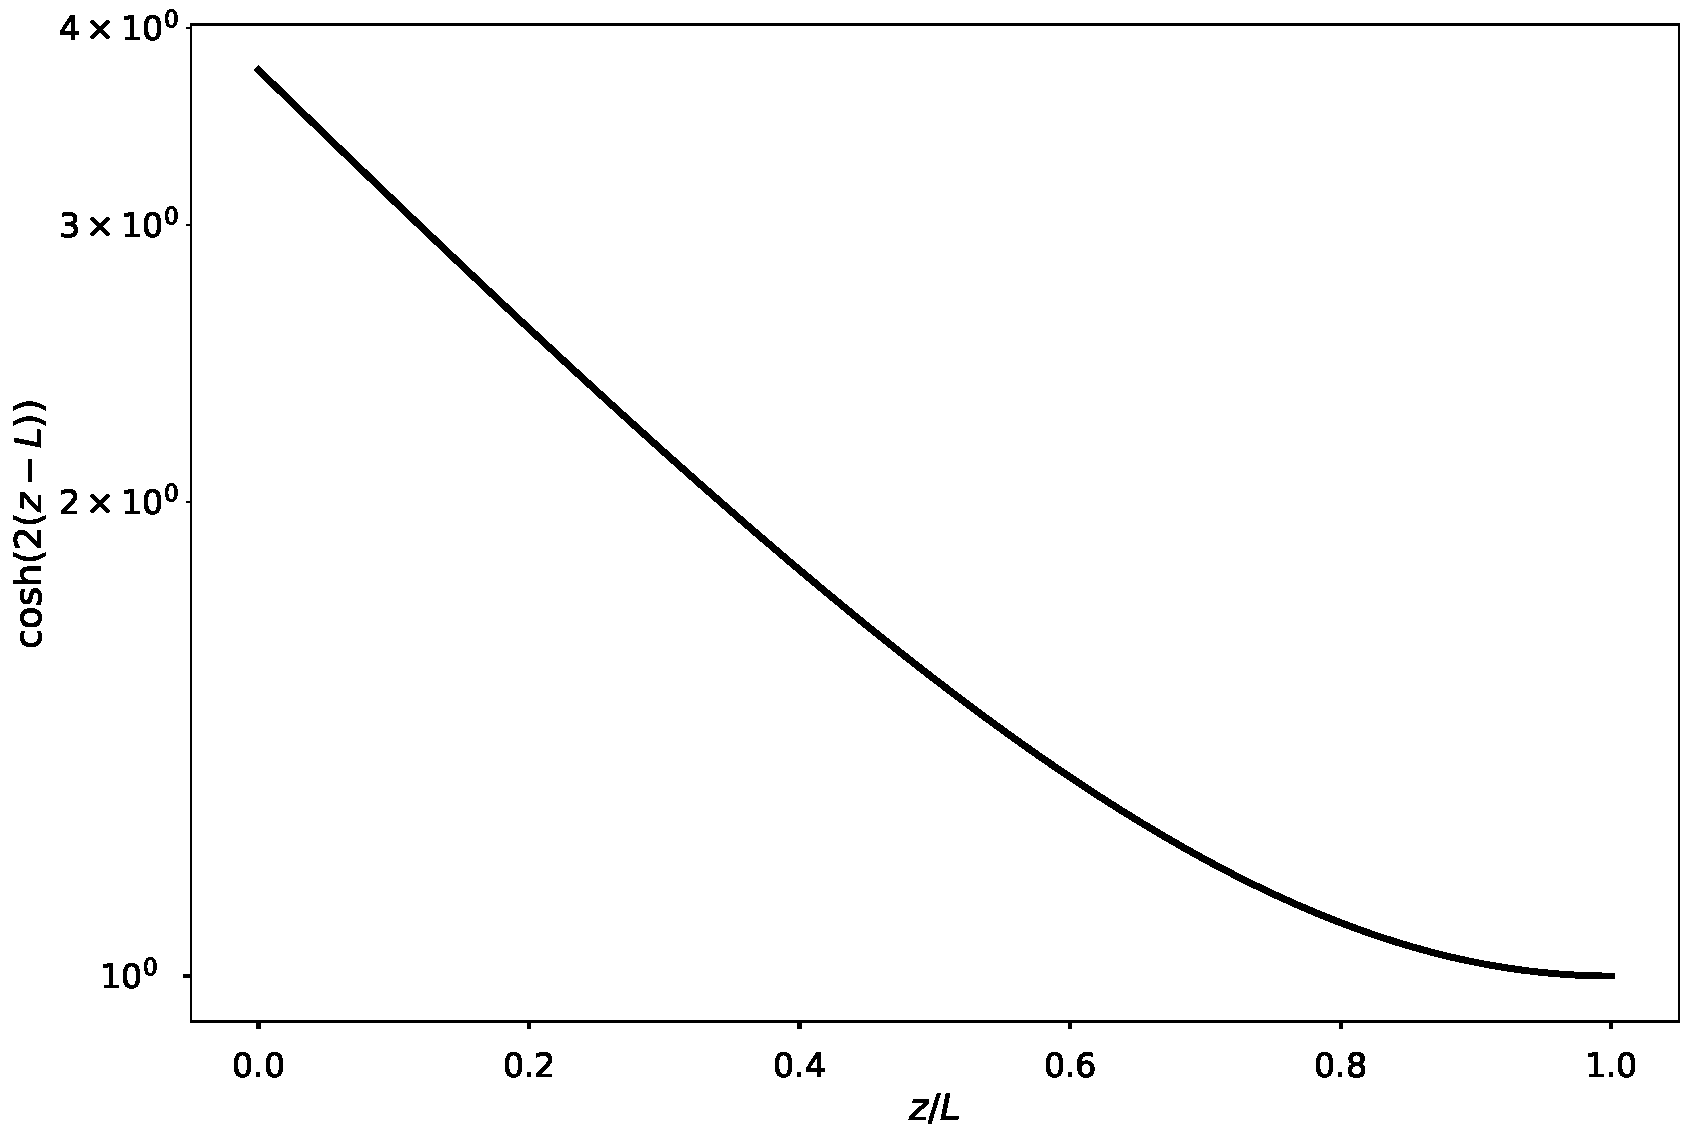
\includegraphics[width=\textwidth]{chapters/assets/halo/cosh.pdf}
    \caption{ An example of $\cosh(2\delta(z-L))$ with $\delta=1$, and $L=5$. This function always reach the minimium at $z=L$.}
    \label{chap:halo-sec:line-sym-fig:cosh}
\end{figure}


We expect the numerical calculations bare the same behavior that the instability leads to no growth but decrease in flavor conversion, assuming the neutrinos start from electron flavor. The result indeed confirms it. Fig.~\ref{chap:halo-sec:line-sym-fig:mu-1.0-reflection-0.07} is an example of it.

\begin{figure}[htbp]
    \centering
    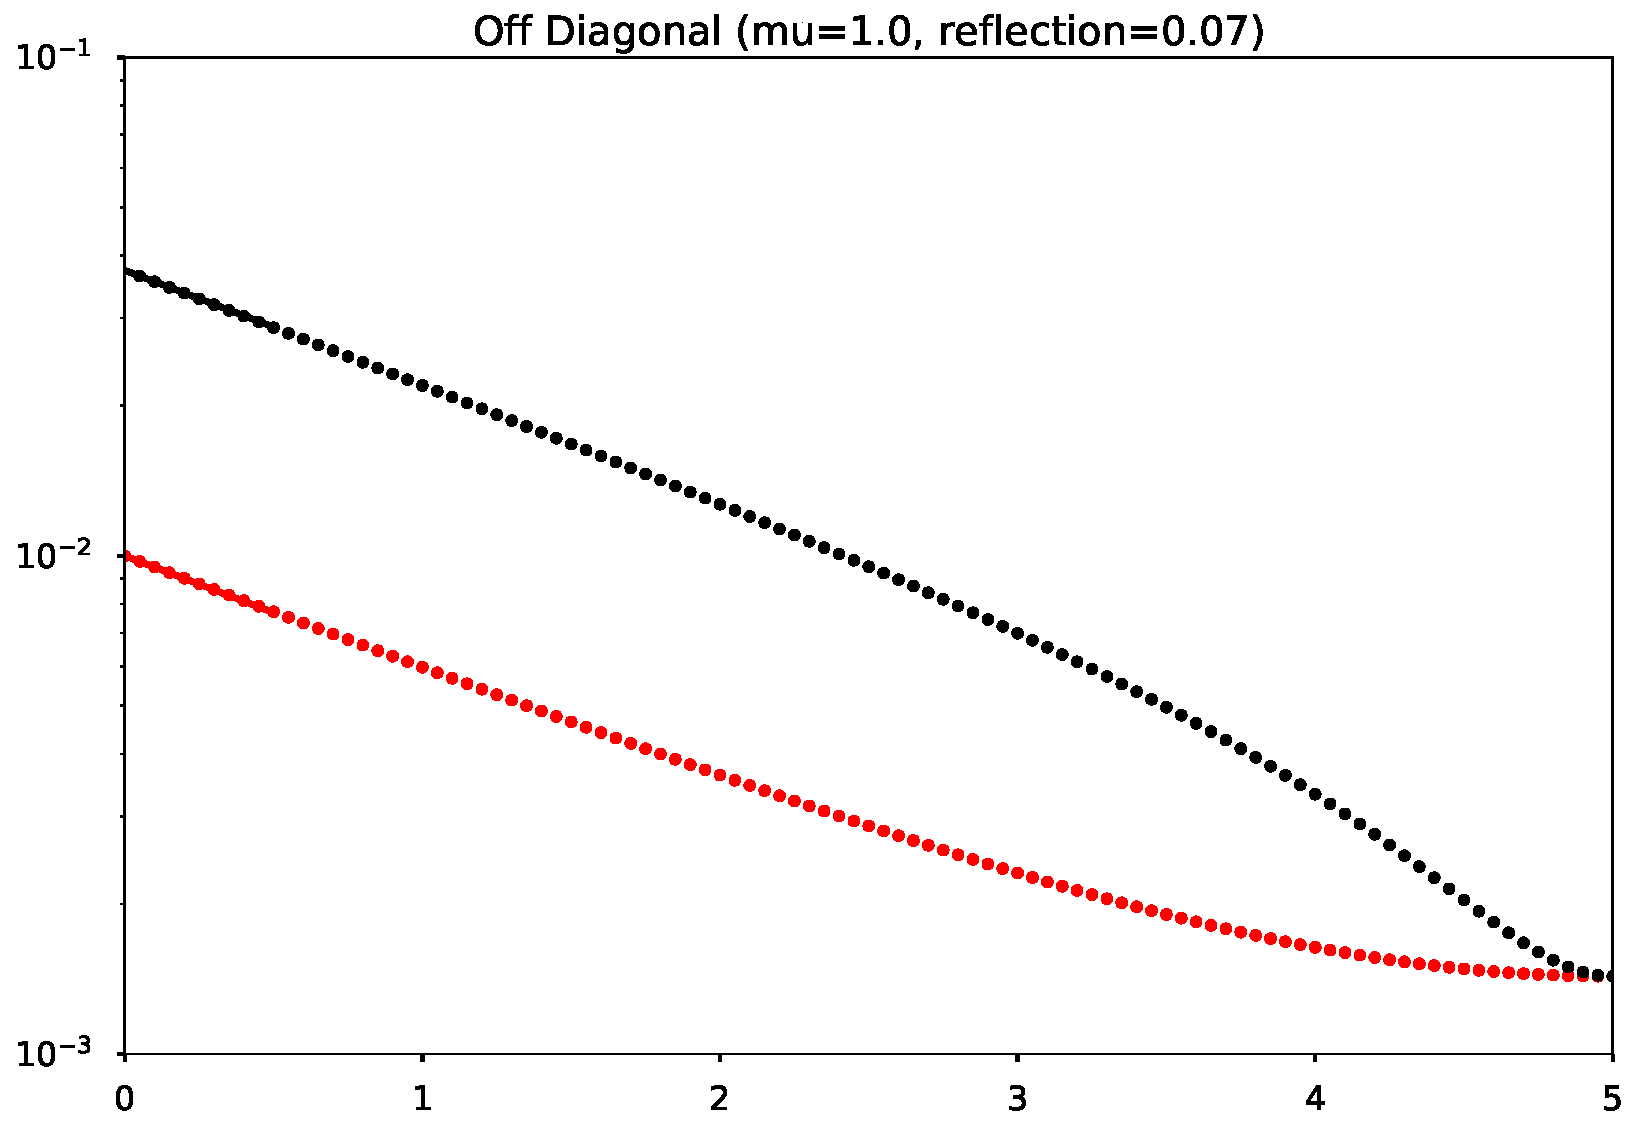
\includegraphics[width=\textwidth]{chapters/assets/halo/mu-1-reflection-0p07.pdf}
    \caption{Absolute value of off diagonal element for $\mu=1.0$, $R=0.07$, $L=5$, with normal hierarchy. The red dots are for the forward beam and the black dots are for the backward beams. The lines are indicating the predictions of linear stability analysis.}
    \label{chap:halo-sec:line-sym-fig:mu-1.0-reflection-0.07}
\end{figure}

For linear stability analysis, I usually identify real characteristic values of the linearized equation of motion. In bipolar model as explained in Sec.~\ref{chap:app-sec:bipolar}, real characteristic values of the equation of motion indicates exponential growth, while it always indicates exponential decrease in this simplified halo problem. 

I expect that only normal hierarchy has an instability region which is trivial since I noticed that the backward beam is acting like antineutrino beams but with different hierarchies.
\begin{align}
 i \partial_t \mathbf s_F &= \mathbf s_F \times (\mathbf {H}_v +R \mu \mathbf s_B) \\
   i\partial_t \mathbf s_B &= \mathbf s_B \times (- \mathbf H_v - \mu \mathbf s_F) .
\end{align}
Compare to Eq.~\ref{chap:app-sec:bipolar-eqn:flavor-isospin-eom}, I notice that 
the reflected beam works as an antineutrino beam but the system becomes the opposite hierarchy compared to bipolar model. I find the instability regions in Fig.~\ref{chap:halo-sec:line-sym-fig:instability-regions}.


\begin{figure}[htbp]
    % \centering
    \minipage{0.49\textwidth}
    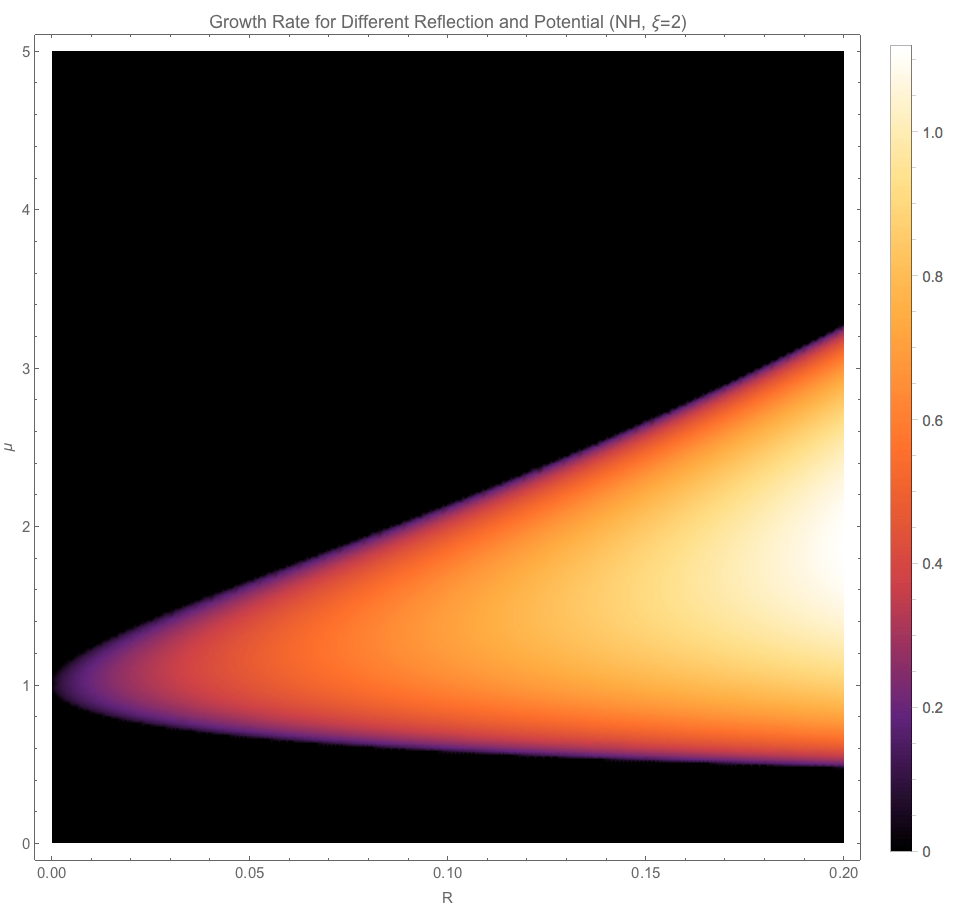
\includegraphics[width=\textwidth]{chapters/assets/halo/growth-rate-mu-refl-nh.jpg}
    \endminipage\hfill
    \minipage{0.49\textwidth}
    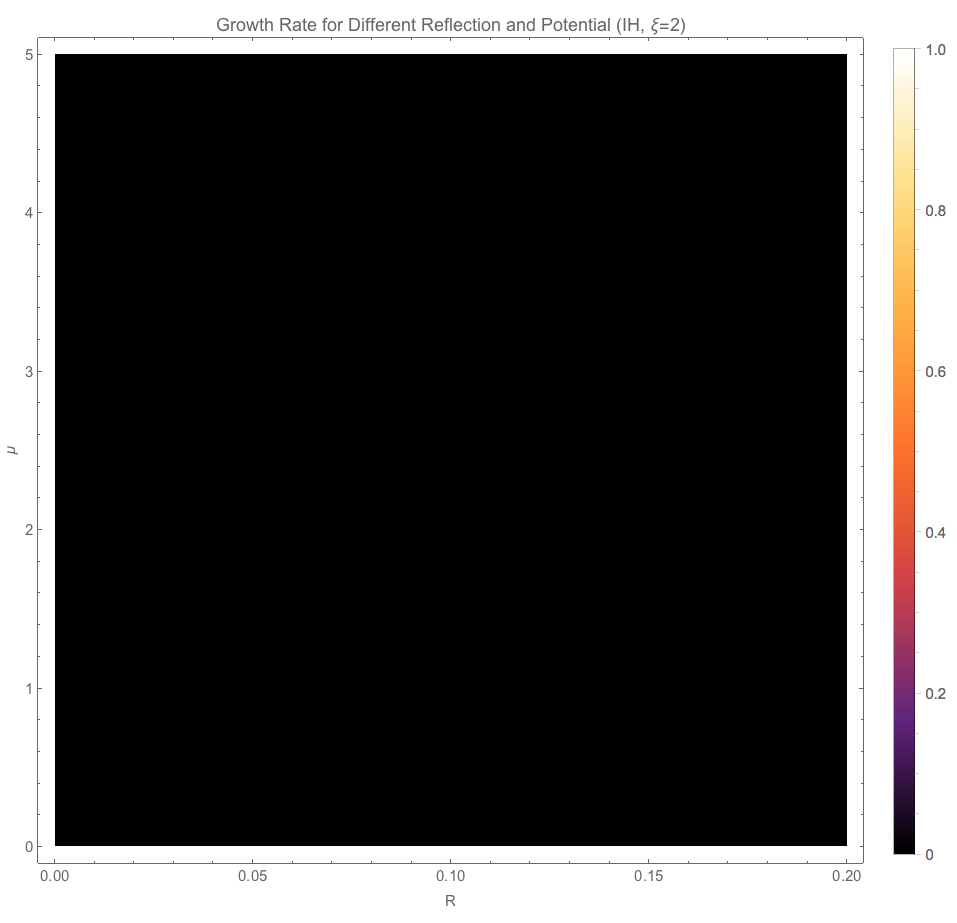
\includegraphics[width=\textwidth]{chapters/assets/halo/growth-rate-mu-refl-ih.jpg}
    \endminipage\hfill
    \caption{Instability regions for normal hierarchy (left) and inverted hierarchy (right) as a function of neutrino potential $\mu$ and reflection coefficient $R$, with vacuum mixing angle set to 0. No instabilities is found in inverted hierarchy.}
    \label{chap:halo-sec:line-sym-fig:instability-regions}
\end{figure}




\subsection{Two Beams Model with Reflection}

The model is naturally extended to a two beams model including both neutrinos and antineutrinos. The configuration is exactly the same as shown in Fig.~\ref{chap:halo-sec:line-fig:line-model}.

As the first step we work out the linear stability analysis. The four equations of motion are
\begin{align}
    i \partial_z \rho_1 = & [ H_1, \rho_1 ], \\
    i \partial_z \rho_2 = & [ H_2, \rho_2 ], \\
    -i \partial_z \rho_3 = & [ H_3, \rho_3 ], \\
    -i \partial_z \rho_4 = & [ H_4, \rho_4 ],
\end{align}
where ${}_1$ and ${}_2$ are the quantities for two forward beams while ${}_3$ and ${}_4$ are the quantities for the corresponding backward going beams. For the purpose of this analysis we set $\theta_v = 0$. The Hamiltonians are
\begin{align}
    H_1 =& -\eta \omega_v \sigma_3 + g_2 \chi_- \mu_2 \rho_2 + g_2 \chi_+ R \mu_2 \rho_4 + g_1 \chi_1 R \mu_1 \rho_3, \\
    H_2 =& \eta \omega_v \sigma_3 + g_1 \chi_- \mu_1 \rho_1 + g_2 \chi_2 R \mu_2 \rho_4 + g_1 \chi_+ R \mu_1 \rho_3, \\
    H_3 =& -\eta \omega_v \sigma_3 + R g_2 \chi_- \mu_2 \rho_4 + g_2 \chi_+\mu_2 \rho_2 + g_1 \chi_1 \mu_1 \rho_1, \\
    H_4 =& \eta \omega_v \sigma_3 + R g_1 \mu_1 \chi_- \rho_3 + g_1 \chi_+ \mu_1 \rho_1 + g_2 \chi_2 \mu_2 \rho_2.
\end{align}

I have defined 
\begin{align*}
    \chi_+ = & 1 - \cos ( \theta_1 + \theta_2 ), \\
    \chi_- = & 1 - \cos ( \theta_1 - \theta_2 ), \\
    \chi_1 = & 1 - \cos ( 2\theta_1 ), \\
    \chi_2 = & 1 - \cos ( 2\theta_2 ),
\end{align*}
and $g_i$ represents the energy spectrum of the neutrinos and $\eta$ stands for the hierarchy.

% Linear stability analysis can be done using computer.

\section{\label{chap:halo-sec:num}Relaxation Method for Neutrino Halo Problem}


We choose a relaxation method scheme to solve this non-local boundary value problem numerically. To begin with, we write down the discretization scheme.
\begin{align}
    \rho(t+\Delta t) &= \left[  \cos( 2 h \Delta t)\rho_n -  2 u_i \rho_i u_n \right]\sigma_n \\
    &= \left[  \cos( 2 h \Delta t) \rho_n +  2 \sin^2(h \Delta t) u'_i \rho_i u'_n \right]\sigma_n
\end{align}
The reason that we use fixed step size for this problem is that it's easier to calculate the neutrino self-interactions on such fixed grids. The algorithm is described as
\begin{enumerate}
    \item
Calculate forward beam using 0 backward beam;
\item
Calculate backward beam and forward beam together using the state of beams from the previous step current counter beams;
\item
Repeat the previous step until the state of the beams reach equilibrium.
\end{enumerate}
To speed up the calculations, I also implemented OpenMP for parallel computing. The code is tested using vacuum oscillations (shown in Fig.~\ref{chap:halo-sec:num-fig:compare-vac-bipolar}) and bipolar models. The reason that we still have conversions is because of the vacuum term, which is additional to linear stability analysis. It is also proven to reach equilibrium quickly as shown in Fig.~\ref{chap:halo-sec:num-fig:relax-color}. 

\begin{figure}[htbp]
    \minipage{\textwidth}
    % 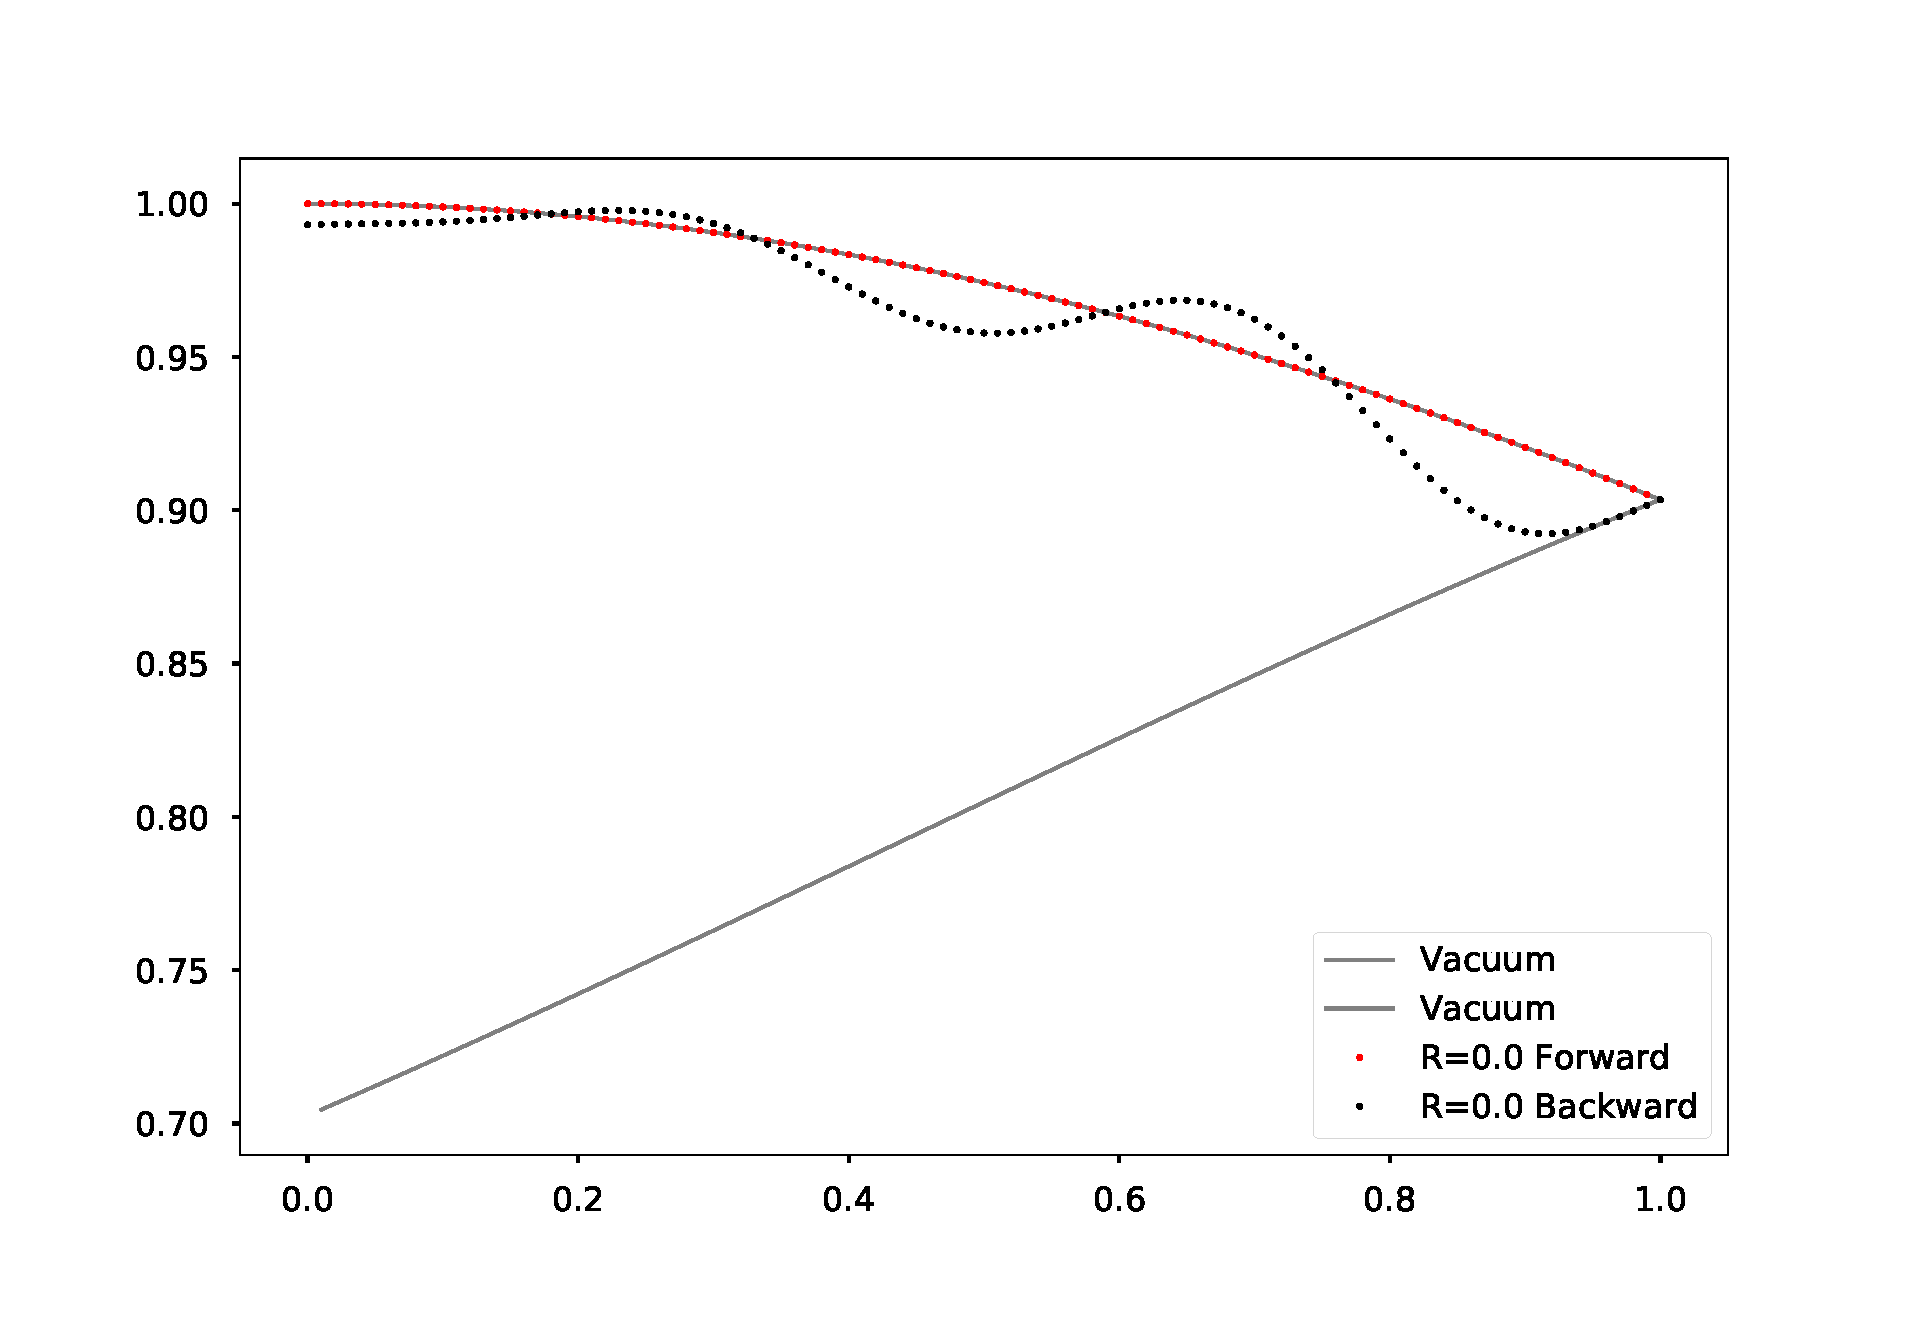
\includegraphics[width=\textwidth]{chapters/assets/halo/halo-mu-4-compare-vac.pdf}
    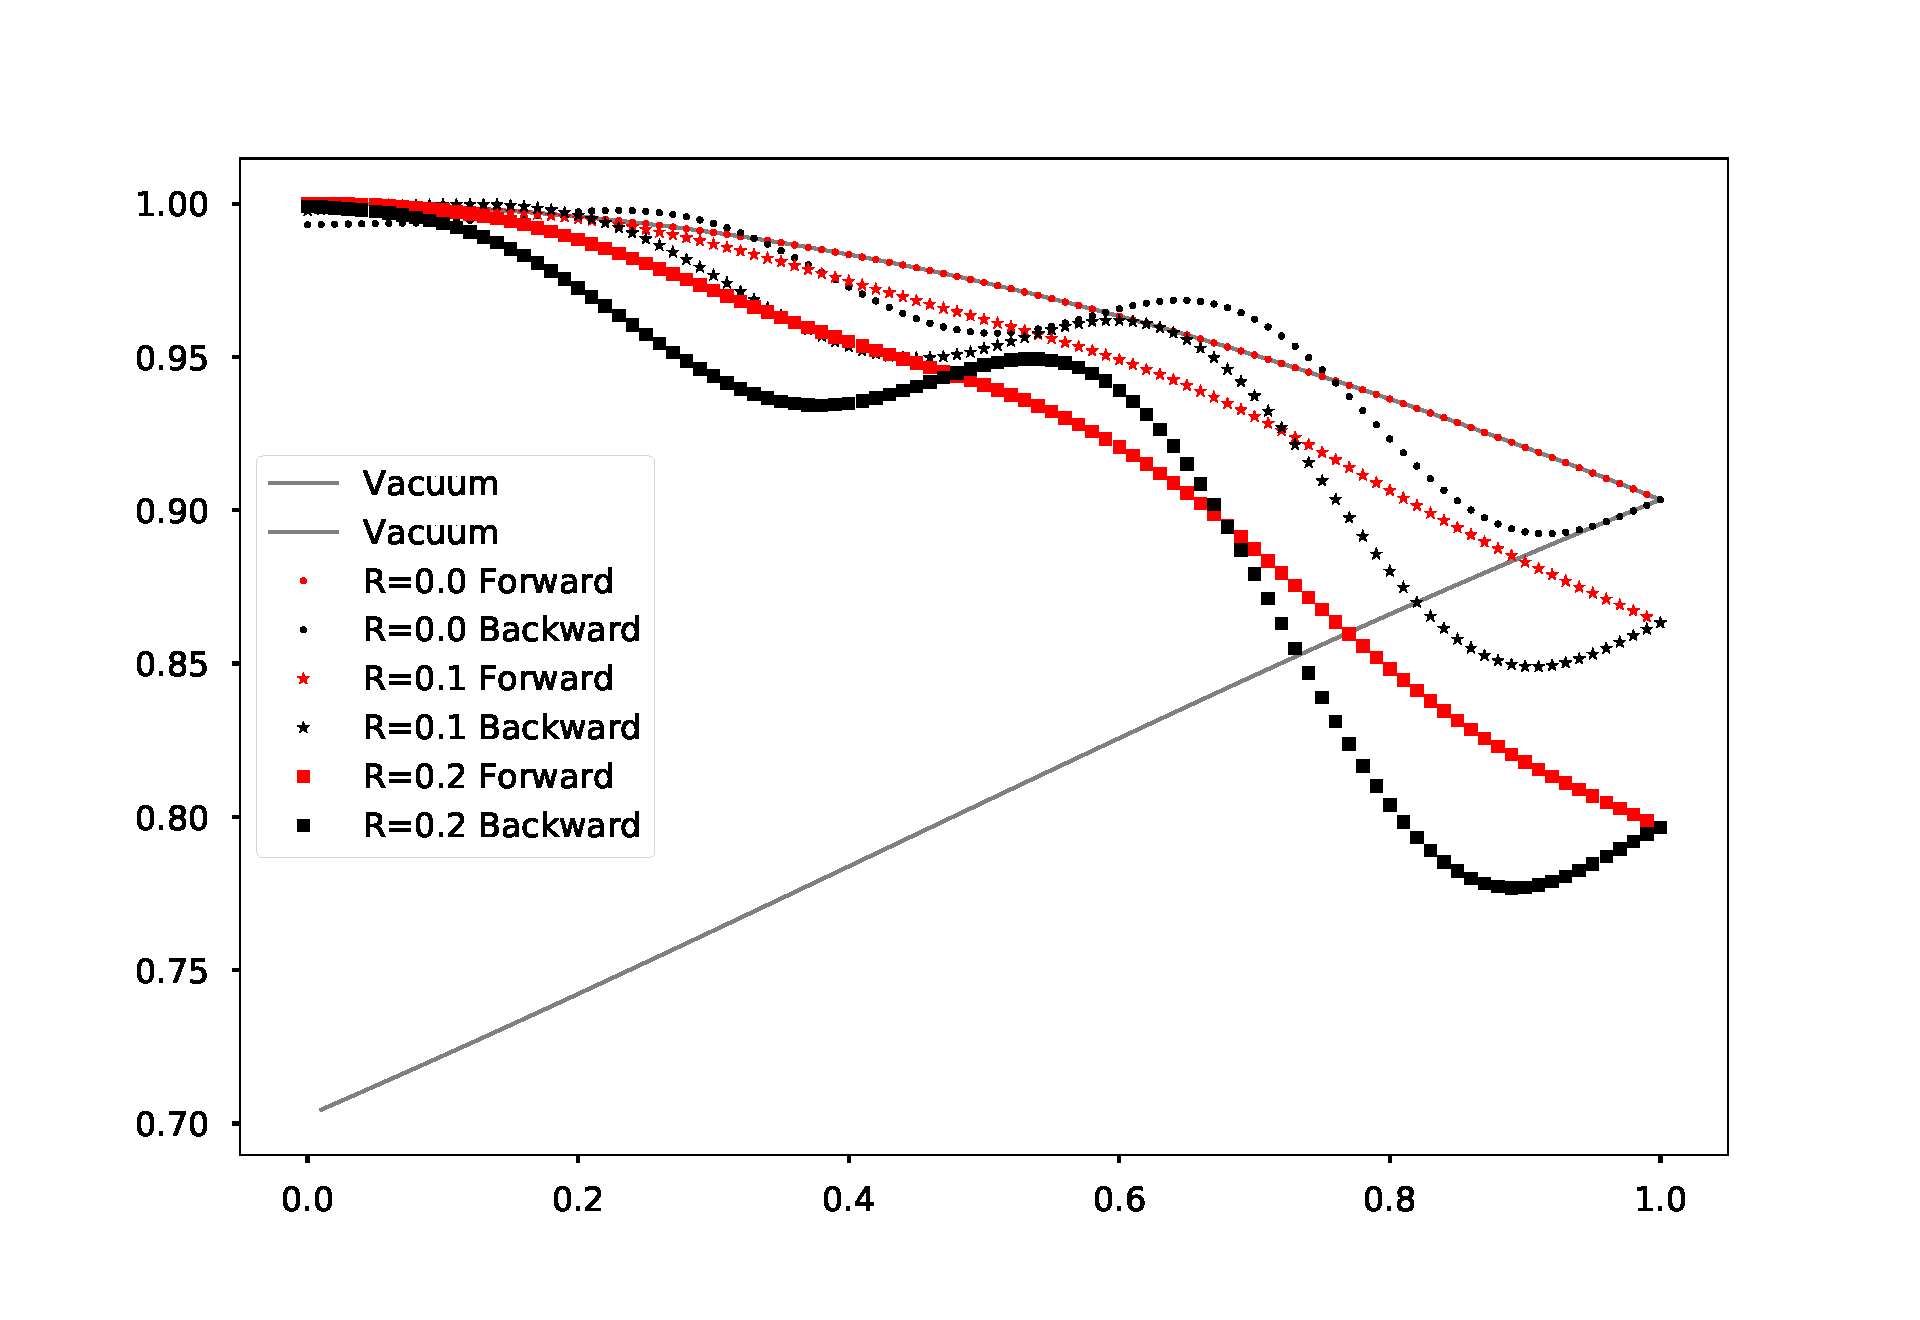
\includegraphics[width=0.49\textwidth]{chapters/assets/halo/halo-mu-4-r-multiple.pdf}
    \endminipage\hfill
    \minipage{\textwidth}
    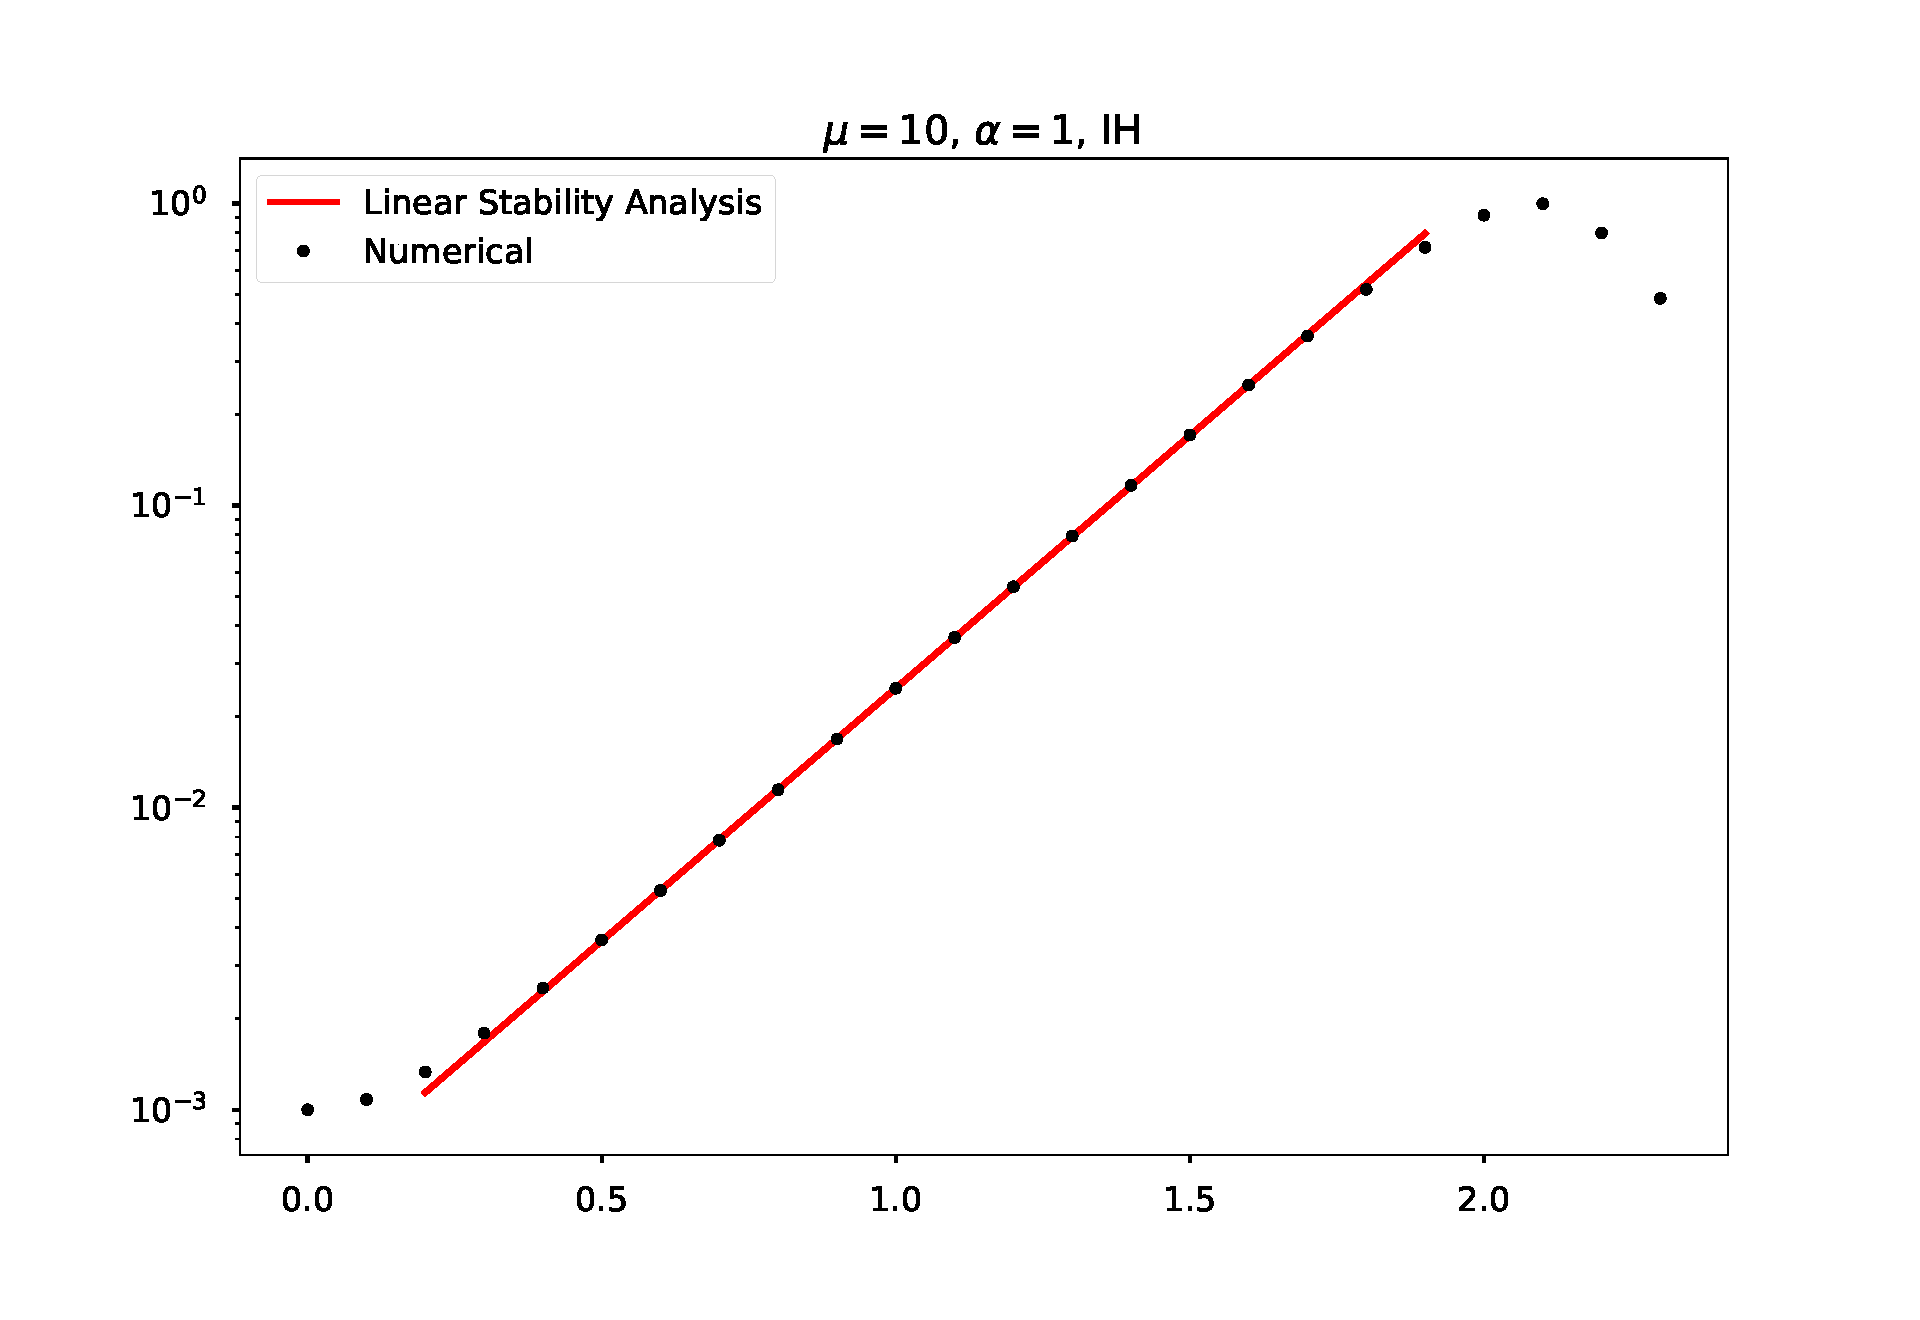
\includegraphics[width=0.49\textwidth]{chapters/assets/halo/halo-mu-4-compare-bipolar.pdf}
    \endminipage\hfill
    \caption{The left panel validates code by setting reflection to zero and approach vacuum for single forward beam. Meanwhile, we notice that for nonzero reflections, more conversion is done, which makes sense due to the similarity between $R$ and the asymmetry parameter $\alpha$ in bipolar model. The right panel validates the code by setting reflection to zero and compare with bipolar model for two beams case, where the slope is matching the theoretical value $3.85$.}
    \label{chap:halo-sec:num-fig:compare-vac-bipolar}
\end{figure}

\begin{figure}[htbp]
    \centering
    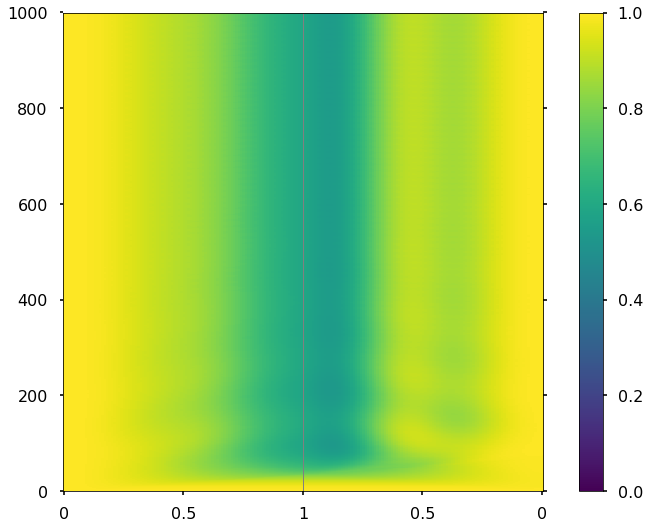
\includegraphics[width=0.8\textwidth]{chapters/assets/halo/relax-color.png}
    \caption{Relaxation method reaches equilibrium after some steps. The horizontal axis is the $z$ direction while the vertical axis is the number of iteration steps. The color indicates the survival probability for electron flavor. This calculation sets $\mu = 4$, $R=0.2$, and is done within range $[0,1]$. Equilibrium is reached around step 400 and the neutrino states stays in equilibrium.}
    \label{chap:halo-sec:num-fig:relax-color}
\end{figure}





%%%%%%%%%%%%%%%%%%%%%%%%%%%%%%%%%%%%%%%%%%%%%%%%%%%%%%%%%%%%%%%%%%%%%%%%%
%%%%%%%%%%%%%%%%%%%%%% Conclusion %%%%%%%%%%%%%%%%%%%%%%%%%%%%
%%%%%%%%%%%%%%%%%%%%%%%%%%%%%%%%%%%%%%%%%%%%%%%%%%%%%%%%%%%%%%%%%%%%%%%%%


\section{\label{chap:collective-sec:conclusion}Conclusion}


The dispersion relations can be extracted from the linearized form of the equation of motion for collective neutrino oscillations. The dispersion relation becomes quadratic for neutrino emission with two zenith angles. Thus two solutions should be found for $\omega$ and $k$. The dispersion relations are hyperbolas and the gaps between the lines corresponds to instabilities. However, this correspondence doesn't hold for neutrinos emitted from more zenith angles. For more realistic spectrum, I have proved that instabilities propagate in regions of either $\omega>0$ or $\omega<0$ and never cross $\omega=0$. Hence the dispersion relation gaps should be defined as gaps between the dispersion relation curves and the axis $\omega=0$ instead of the dispersion relation curves. I have also showed that instabilities is not necessarily shown as gap in dispersion relations for neutrino emission with more than two zenith angles and box spectrum with crossing. Through the discussions, I demonstrated that the relation between dispersion relation gaps and instabilities should be used with caution.


The second problem discussed in this chapter is the halo problem, which brings in more complexities to the neutrino oscillations. In the spirit of numerical methods, I developed a parallelable relaxation method, using C++ and OpenMP. Both the analytical and numerical results showed that for the two realms, either single forward beam or two forward beams, the results are compared with bipolar model. This simple model is very similar to the bipolar model thus I can perform linear stability analysis and verify my numerical method. The reflection indeed may enhance the flavor conversions but it is not a new type of instability. Future work should be done to explore the effect of symmetry breaking and multiple emission beams.
